% Do not forget to include Introduction
%---------------------------------------------------------------
\chapter{Úvod}
% uncomment the following line to create an unnumbered chapter
%\chapter*{Úvod}\addcontentsline{toc}{chapter}{Introduction}\markboth{Introduction}{Introduction}
%---------------------------------------------------------------
\setcounter{page}{1}

% The following environment can be used as a mini-introduction for a chapter. Use that any way it pleases you (or comment it out). It can contain, for instance, a summary of the chapter. Or, there can be a quotation.
%\begin{chapterabstract}
%	\lipsum[1]
%\end{chapterabstract}

%\section{Motivace}
\section{Cíle práce}
Prvním důležitým cílem práce je analyzovat použitelnost nově nastupující technologie na poli vývoje multiplatformního UI a otestovat, jaké
nové principy přináší. Dále tuto technologii porovnat s ostatními frameworky pro tvorbu multiplatformního UI a pokusit se
rozebrat důležité principy, na kterých jsou tyto technologie postaveny. 

Další podstatným cílem je vytvoření aplikace, která tuto technologii implementuje a zaměření se při tom na slabé stránky, 
které aktuálně multiplatformní UI provází.

Posledním hlavním cílem je vytvořenou aplikaci otestovat a zhodnotit použitelnost daného frameworku v praxi.

\section{Stručný přehled obsahu práce}
V rámci se práce zabývá otázkou co to vlastně multiplatformní vývoj je, proč se jím zabývat a jakých platforem se může týkat.
Dále je probrána otázka v jakých případech se vyplatí aplikovat multiplatformní UI a na jakých zařízeních. 

%a porovnání vazby s UI s logikou daného aplikace vůči multipaltfomovodsti.



%kdy multiplatformí vývoj nemá smysl (vyfocení závady)


Jaké jsou výhody a nevýhody multiplatformních aplikací  v porovnaní s nativními aplikacemi.

Existujícími frameworky a jich porovnáním s Compose Multiplatform.

Detailně rozebrána architektura Compose Multiplatform jak framework funguje a jaké další technologie jsou potřeba k smysluplné implementaci tohoto
frameworku.

Dále je se práce zabývá návrhem a následnou tvorbou multiplatformního UI pomocí frameworku Compose Multiplatform.

V v jedné z posledních části se týká možností testování takto vytvořeného UI a následného testování UI na naimplementované aplikaci.

je věnován shrnutí celého procesu implementace a vyzdvižení naskytlých problémů a výhod oproti nativnímu případně jiným multiplatformním frameworkům



Obecně něco o multiplatformním vývoji.

\section{Definice multiplatformního vývoje UI}

Technologie sloužících k tvorbě multiplatformních UI umožňují vývojářům vytvářet jednotná uživatelské rozhraní, 
která mohou být nasazena na různé platformy, jako jsou mobilní zařízení, webové prohlížeče nebo desktopové aplikace. 
Cílem je dosáhnout jednotného uživatelského zážitku bez nutnosti psát a udržovat oddělené kódy pro každou platformu.


\section{Důvody multiplatformního vývoje a sdíleného UI}

Mezi primární důvody vedoucí firmy a jednotlivce k vývoji multiplatformních aplikací patří především
snížení nákladů na vývoj a následně také na údržbu. Jednodušší dosažení konzistentního vzhledu
na různých platformách nebo například možnost znovu používat komponenty UI na různých platformách.

Mezi další důvody může například patřit možnost rychlejších aktualizací, jelikož nové funkce mohou být 
implementovány jednotně a rychle na všech platformách. 

\section{Uplatnění multiplatformního vývoje a sdíleného UI}

I přesto že tato práce je věnováno tvorbě UI, tak nesmí být opomenuta aplikační logika, které se za ním skrývá a má UI vliv naopak. Dále zde
hrají velkou roli případy užití, které mají na jednotlivá a UI vliv a při multiplatformním vývoji je třeba dbát na jelikož né každá aplikace
je z tohoto pohledu vhodná pro multiplatformní


Aktuálně největší uplatnění použití uplatnění multiplatformního UI nabízí mobilní vývoj, který díky multiplatformním frameworkům umožňuje vývoj
aplikací na platformami Android a iOS současně. 
To že tomu tak je je primárně díky hlavnímu důvodu vedoucí firmy k multiplatformnímu vývoji aplikací a tím je snížení nákladu na vývoj.

Výběr těchto platforem je vhodný především díky podobnostem majících na návrh multiplatformního UI vliv jako je například velikost obrazovky.

I přesto, že multiplatformní frameworky umožňují implementaci multiplatformním UI na většinu nejvíce používaných platforem jako je Android, iOS,
automotive, TV, wear OS, tak né vždy je těchnoto možností využít.

Z pohledu UI mají ty platformy často jiné velikosti obrazovek, jine možnosti ovládaní a proto, je často multiplatformní UI a často i veškerá logika
implementována konkrétně pro danou platformu nebo typ zařízení.

Je proto vždy nutné vědět jaký typ aplikace bude z pohledu aplikační logiky implementován, jaké budou jeho způsoby užití a na jakých platformách
bude daná aplikace implementována.

Obecně tedy nelze říci, že efektivita implementace multiplatformních aplikaci se může dle těchto požadavků výrazně lišit.






%Větší dosah jelikož díky sdílení UI lze dosáhnout většího dosahu, protože aplikace mohou být dostupné 
Tato kapitola je zaměřena na představení multiplatformních frameworků, porovnání mezi nimi. 


\chapter{Analýza}

\section{Přehled existujících frameworků}
Mezi aktuálně nejpopulárnější multiplatformní frameworky jednoznačně patří Flutter a React Native. \cite{crossPlatformFrameworksStats}
V následujících kapitolách jsou proto tyto nejpoužívanější frameworky podrobněji rozebrány a u každého z nich jsou vybrány 
důležité vlastnosti, které jsou pro tyto frameworky typické. 

Jednotlivé frameworky jsou seřazeny postupně od nejstaršího
po nejmladší, což umožňuje lepší náhled na to, jak se jednotlivé frameworky v čase vyvíjely. Pro lepší ilustraci byla také zvolena 
i podobná struktura jednotlivých kapitol, čehož bylo možné docílit díky mnoha společnými rysům napříč frameworky.

%---------------------------------------------------------------
\subsection{React Native}
%---------------------------------------------------------------
React Native byl jedním z prvních frameworků pro tvorbu multiplatformního UI a do jisté míry ovlivnil i ostatní popisované
frameworky. Jeho vývoj započal ve společnosti Facebook během interního hackaton projektu a první jeho oficiálně publikovaná
verze vyšla začátkem roku 2015. \cite{reactNativeHistory}
Nyní se jedná o open-source framework, kde jeho hlavním cílem je umožnit vývojářům vytvářet nativní mobilní aplikace 
pro platformy Android a iOS z jednoho společného kódu napsaného v jazyce JavaScript nebo TypeScript.

\section*{Klíčové vlastnosti React Native}

\myparagraph{Komponentní architektura} 
React Native využívá komponentní architekturu, která vývojářům umožňuje 
vytvářet znovupoužitelné komponenty. \cite{reactNativeComponents} Tato architektura je jednak založena na obecných
React komponentách, ale zároveň také na React Native specifických komponentách, které se dále dělí na takzvané core
komponenty, komponenty vytvořené komunitou či vlastní nativní komponenty. \cite{reactNativeComponents}

% // todo komponenty prekladane na nativni 
    
\myparagraph{Deklarativní zápis UI}
React Native stejně jako React pro webové aplikace využívá pro zápis UI deklarativní způsob, 
při kterém využívá JSX (JavaScript XML) syntaxe k popisu struktury UI komponent. \cite{reactNativeJSX}
Takto zapsané UI lépe reflektovalo aktuální stav aplikace.
Tento způsob zápisu začal na mobilních platformách růst popularitě právě díky Reactu Native, který po svém uvolnění v roce 2013 
defacto nastartoval éru deklarativního zápisu UI na mobilních platformách. \cite{declarativeUIHistory}

\myparagraph{Fast Refresh} 
Fast Refresh je v funkce, která vývojářům umožňuje okamžitě vidět výsledky provedených 
změn v kódu bez nutnosti znovu sestavení aplikace. \cite{reactNativeFastRefresh}

\myparagraph{JavaScript/TypeScript} 
Aplikační logika v React Native se píše v jazyce JavaScript nebo TypeScript, 
což usnadňuje snadnou integraci s existujícími webovými technologiemi. \cite{reactNativeFundamentals}

\myparagraph{Rozsáhlá komunita} 
React Native má rozsáhlou komunitu vývojářů, což vede k bohatému ekosystému 
třetích stran, včetně mnoha dostupných knihoven a modulů. \cite{reactNativeComunity}

\myparagraph{Expo framework} 
Pro ještě snazší start vývoje poskytuje React Native Expo framework, který 
zjednodušuje proces vývoje a umožňuje rychlé prototypování. \cite{reactNativeExpo}

\subsection*{Architektura frameworku React Native}

React native do roku 2022 využíval architekturu založenou na návrhového vzoru Bridge, který spojoval kód napsaný v JavaScriptu s nativní kódem určeným pro danou platformu. 
Tyto dva celky byly spuštěny na souběžných vláknech a komunikovaly spolu pomocí zasílání serializovaných zpráv. Časem se ale ukázalo, že se tato komunikace
a další její charakteristiky stávají úzkým hrdlem celého systému a byla proto od verze 0.68 nahrazena JavaScriptovým rozhraním zvaným JSI. \cite{reactNativeAboutNewArch}

JSI nově JavaScriptu umožňuje držet referenci na C++ objekty a volat nad nimi potřebné metody. \cite{reactNativeAboutNewArch} Toho využívá nový renderovací systém zvaný \textit{Fabric}, který 
frameworku napomáhá sjednotit renderovací logiku prováděnou v C++ a zlepšit tak interoperabilitu s nativními platformami.

\begin{figure}[H]
  \centering
  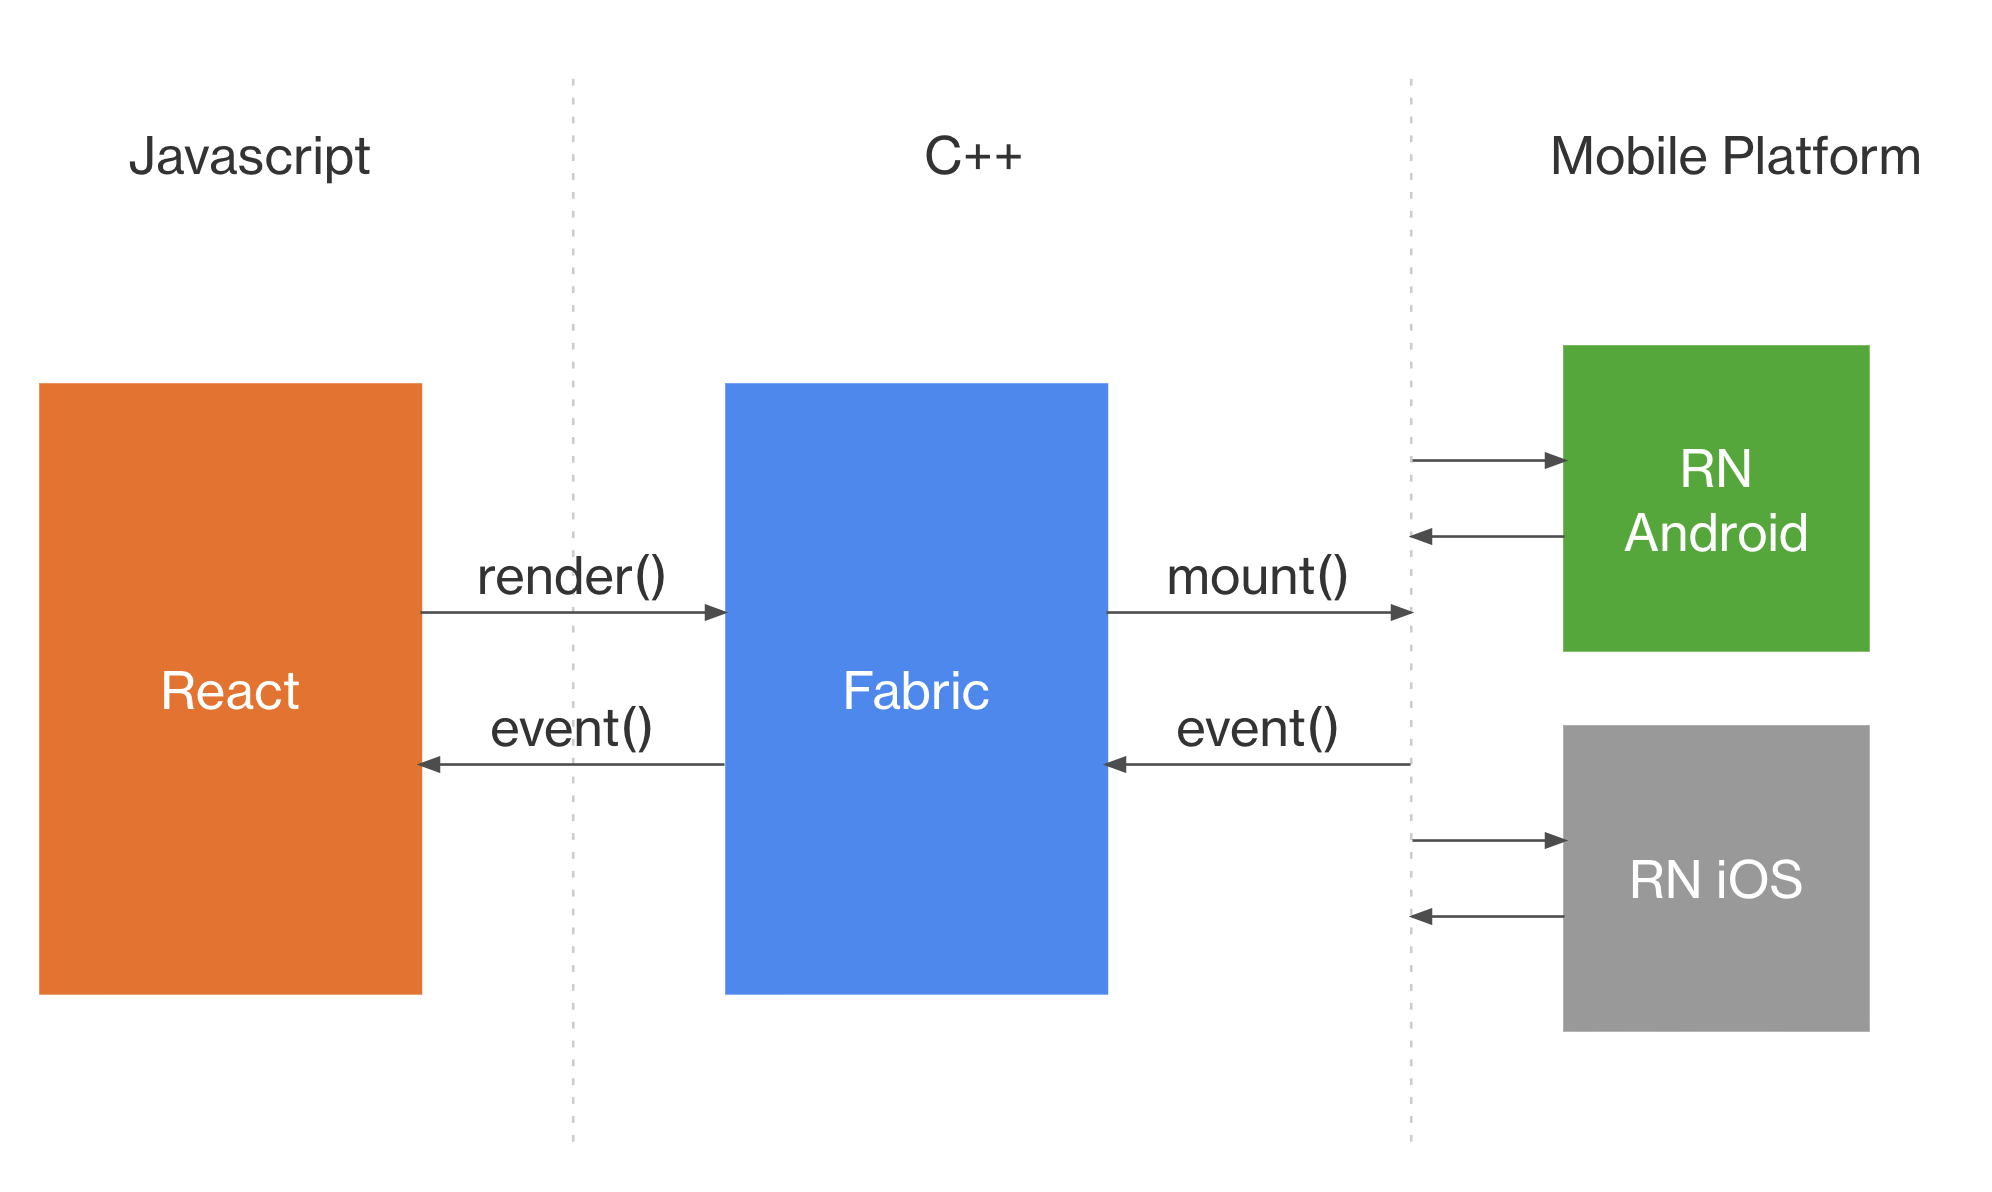
\includegraphics[width=0.85\textwidth]{react-natice-xplat-implementation-diagram.png}
  \caption{React Native }
  \label{fig:react-natice-xplat-implementation-diagram}
\end{figure}

% \begin{figure}[H]
%   \centering
%   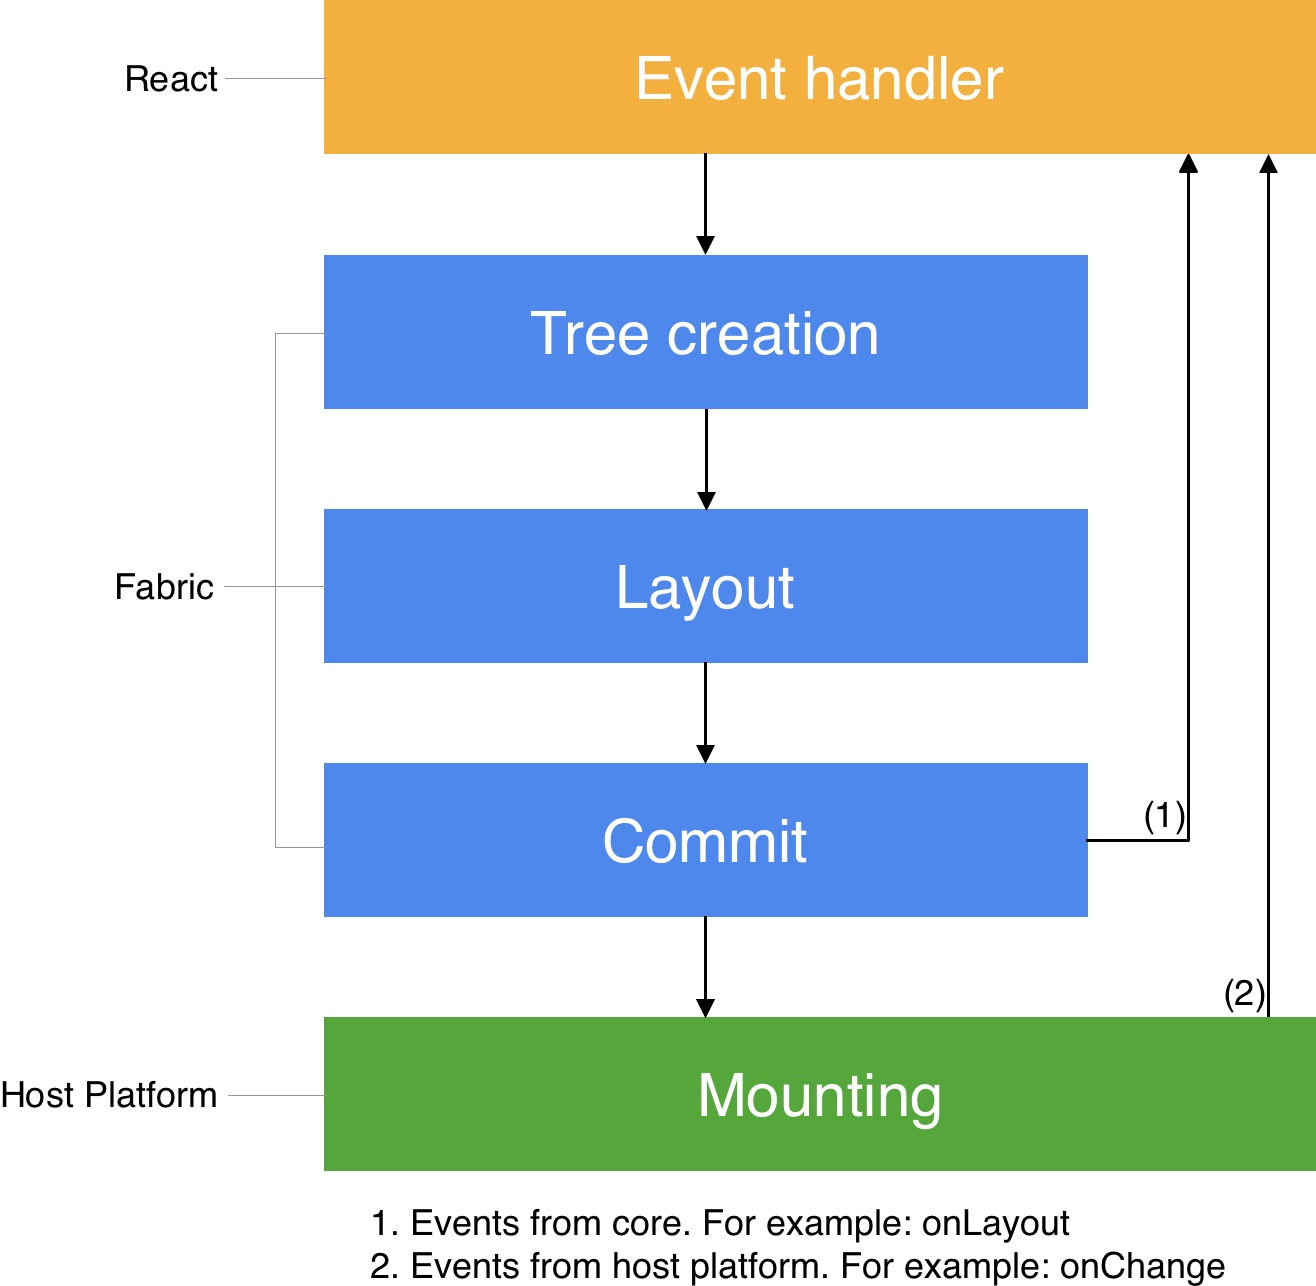
\includegraphics[width=0.55\textwidth]{react-native-data-flow.jpg}
%   \caption{React Native tok dat}
%   \label{fig:react-natice-data-flow}
% \end{figure}


% I přes tyto změny React Native stále využívá systém dvou typů vláken označovaných jako \textit{JavaScript Thread} a \textit{UI Thread} (známé taktéž pod názvem \textit{Main Thread}) 
% mezi které rozděluje práci.


Jak je vidět na obrázku \ref{fig:react-natice-xplat-implementation-diagram}, tak Fabric de facto plní funkci prostředníka, který převádí React 
komponenty na nativní komponenty pro každou platformu. 

Pro lepší představu jak dané komponenty vypadají slouží následující ukázka kódu \ref{lst:reactNativeJSX}.

\begin{lstlisting}[caption={Popis UI komponent pomoci JSX}, label={lst:reactNativeJSX}, language=XML]
function MyComponent() {
  return (
    <View>
      <View
        style={{backgroundColor: 'red', height: 20, width: 20}}
      />
      <View
        style={{backgroundColor: 'blue', height: 20, width: 20}}
      />
    </View>
  );
}
// <MyComponent />
\end{lstlisting}

Na ukázce kódu \ref{lst:reactNativeJSX} jsou použity některé z nejpoužívanějších core komponent, které se při psaní React
Native aplikací používají. \cite{reactNativeComponents} Jak již bylo zmíněno dříve, tak tyto komponenty jsou následně převedeny 
na nativní komponenty pro každou platformu a to jakým způsobem Fabric dané komponenty převádí se dá rozdělit do následujících tří
na sebe navazujících fází: \cite{reactNativeRenderCommitMount}
 
%Na této ukázce je zároveň vidět použití deklarativního zápisu, které bude podrobněji probráno v následující kapitole.

\smallskip

\myparagraph{Render}
Během této fáze se z jednotlivých komponent (React Elementů) sestaví strom elementů v JavaScriptu (viz levá část obrázku \ref{fig:react-native-render-pipeline}) a nad tímto stromem se 
následně spustí rekurzivní redukce, při které dojde k vytvoření nového stromu takzvaného React Shadow Tree. (viz prostřední část obrázku \ref{fig:react-native-render-pipeline})
\cite{reactNativeRenderCommitMount} Ten se skládá z jednotlivých React Shadow Nodes, které reprezentují objekty v C++ a tím přechází tato renderovací fáze do další fáze zvané commit.\cite{reactNativeRenderCommitMount}

\myparagraph{Commit}
V rámci této fáze je pro každý React Shadow Node vypočítána jeho pozice a velikost na koncovém zařízení a díky tomu může renderovací systém
přejít k poslední fázi zvané Mount. \cite{reactNativeRenderCommitMount}

\myparagraph{Mount}
Během této poslední fáze dojde k transformaci \textit{React Shadow Tree} na \textit{Host View Tree} (viz pravá část obrázku \ref{fig:react-native-render-pipeline}) a to tak, že každý \textit{React Shadow Node}
se transformuje na jeho ekvivalent v nativní podobě. \cite{reactNativeRenderCommitMount} Čili například na platformě Android se $<ViewShadowNode>$ přetransformuje na android.view.ViewGroup. \cite{reactNativeRenderCommitMount}

\begin{figure}[H]
  \centering
  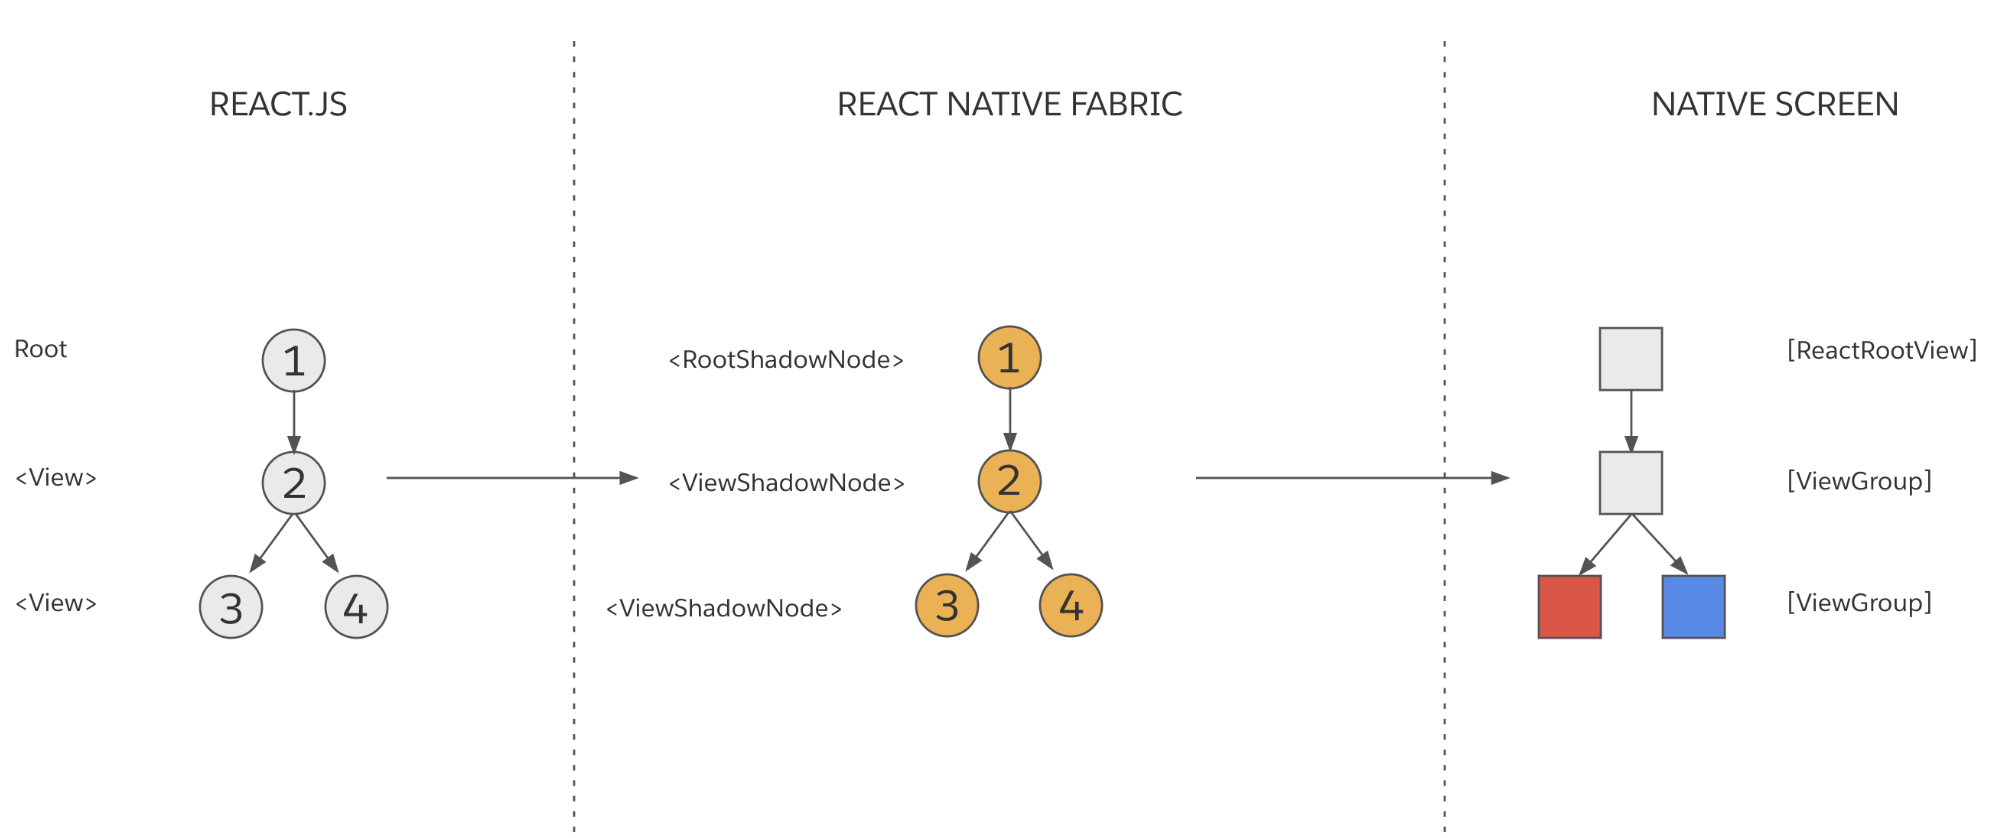
\includegraphics[width=0.99\textwidth]{react-native-render-pipeline.png}
  \caption{React Native vykreslovací fáze}
  \label{fig:react-native-render-pipeline}
\end{figure}

%---------------------------------------------------------------
\subsection{Flutter}
%---------------------------------------------------------------
Flutter je open-source softwarový toolkit pro vývoj uživatelských rozhraní (UI). \cite{flutterfaq} Za vývojem stojí společnost Google a je určený k vytváření nativně kompilovaných 
aplikací pro mobilní zařízení, web a desktop z jednoho zdrojového kódu. \cite{flutterfaq}
Byl vydán v roce 2017 a získal značnou popularitu mezi vývojáři díky svému snadnému použití, flexibilitě a schopnostem tvorby UI.

\subsection*{Klíčové vlastnosti Flutteru}

\myparagraph{UI založené na widgetech} 
Flutter využívá reaktivně deklarativní UI založené na widgetech. \cite{flutterUI} Widgety jsou základními stavebními 
bloky Flutter aplikací, představující vše od strukturálních prvků po stylistické komponenty. \cite{flutterWidgets}

\myparagraph{Hot Reload} 
Další z významných funkcí Flutteru, která významně zrychluje vývojový proces a zvyšuje produktivitu je funkce "Hot Reload". 
Během vývoje běží Flutter aplikace na virtuálním počítači (Dart VM), který díky této funkci umožňuje okamžitě vidět provedené změny
v kódu bez nutnosti úplné rekompilace aplikace. \cite{flutterHotReload} Teprve pro vydání jsou Flutter aplikace kompilovány přímo do strojového kódu, 
ať už jde o instrukce Intel x64 nebo ARM, případně do JavaScriptu pokud jsou cíleny na web. \cite{flutterArchOverview}


\myparagraph{Jeden zdrojový kód pro více platforem} 
S Flutterem mohou vývojáři psát jeden zdrojový kód pro obě platformy Android a iOS, což snižuje dobu vývoje a úsilí 
vynakládané na údržbu. Flutter také rozšířil svou podporu pro cílení webových a desktopových aplikací, umožňující širší dosah s minimálními změnami kódu. \cite{flutter}

\myparagraph{Rozsáhlá sada widgetů}
Flutter poskytuje komplexní sadu přizpůsobitelných widgetů, které usnadňují vytváření složitých a vizuálně 
atraktivních uživatelských rozhraní. Tyto widgety zahrnují vše od základních tlačítek a textových polí až po 
pokročilé komponenty jako jsou grafy a animace.

\myparagraph{Programovací jazyk Dart}
Aplikace vytvořené ve Flutteru jsou psány v jazyce Dart, moderním objektově orientovaném programovacím jazyce 
vyvinutém společností Google. Dart je navržen pro optimální výkon a produktivitu, což ho činí vhodným pro mobilní a
webový vývoj. \cite{dart}

\myparagraph{Způsob renderovaní UI}
Na rozdíl od Reactu Native Flutter nepoužívá platformě specifické komponenty koncových zařízení, ale veškeré UI komponenty (widgety)
renderuje pomocí vlastního renderovacího enginu. \cite{flutterRenderingModel}


\subsection*{Architektura frameworku Flutter} 
Jak je vidět na obrázku \ref{fig:flutter_architectural_layers}, tak architektura Flutteru je rozdělena do tří hlavních vrstev. \cite{flutterArchOverview}
Embedder je vrstva, která umožňuje integrovat Flutter do konkrétních platforem jako je Android, iOS, desktop nebo web. 
Každý embedder obsahuje platformě specifický kód, který je potřebný pro spuštění Flutteru na dané platformě.
Engine je vrstva starající se o vykreslování grafiky, kdykoli kdy je potřeba vykreslit nový snímek. \cite{flutterArchOverview} 
Framework je vrstva, která je používána vývojáři k vytváření uživatelských rozhraní a definování chování aplikace. 
Obsahuje hotové widgety, funkce pro manipulaci s UI a další nástroje pro vývojáře. \cite{flutterArchOverview} 


\begin{figure}[H]
  \centering
  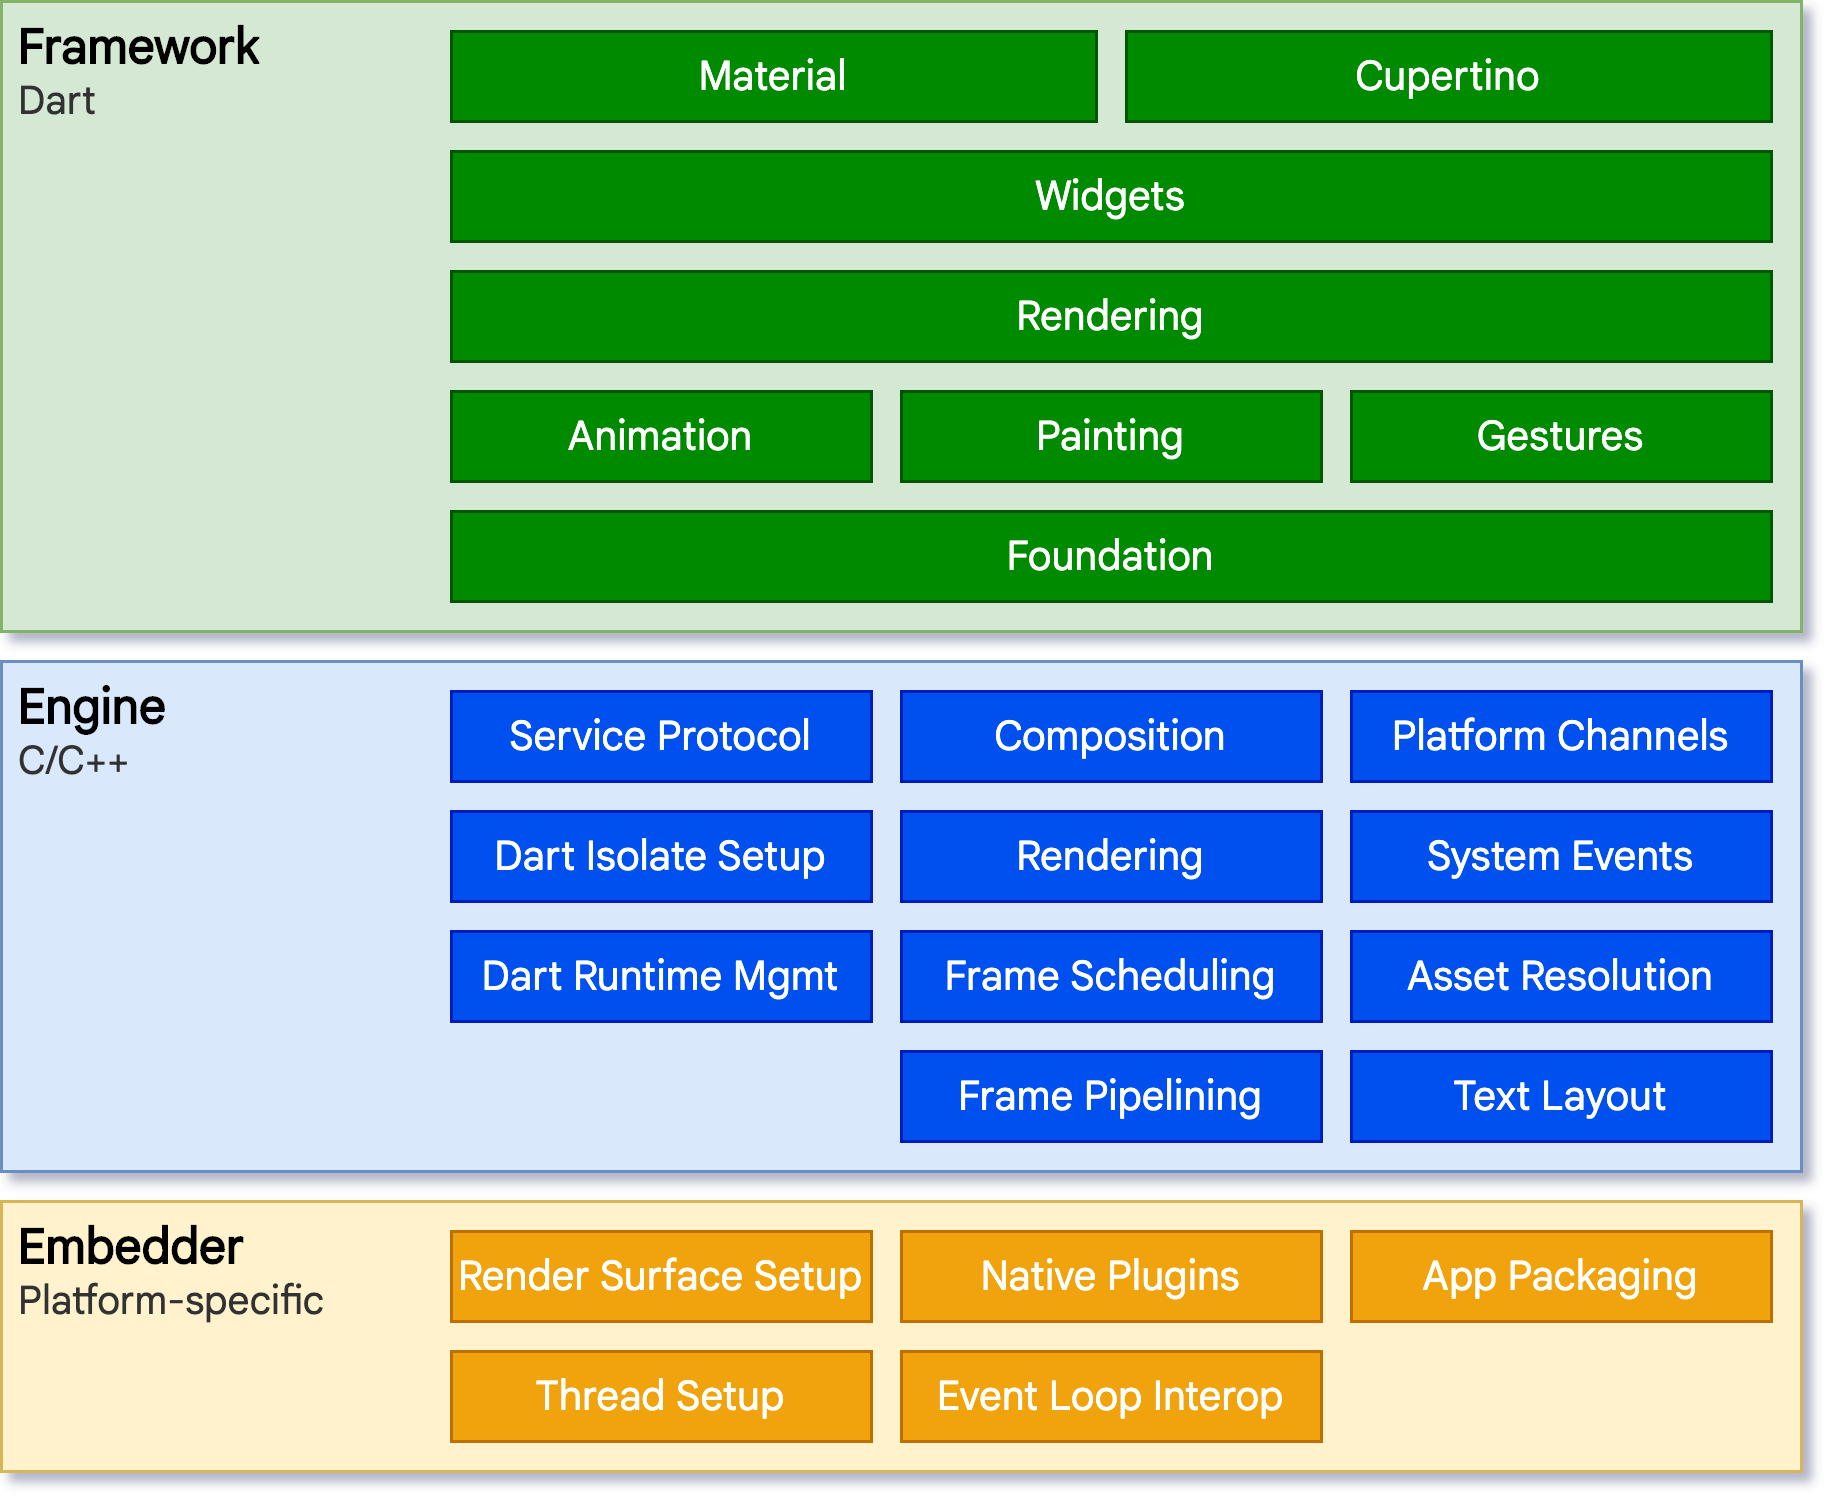
\includegraphics[width=0.85\textwidth]{flutter_architectural_layers.png}
  \caption{Flutter architectural layers}
  \label{fig:flutter_architectural_layers}
\end{figure}

Mezi hierarchicky poslední a neméně důležitou častí tohoto frameworku jsou platformě specifické knihovny Material and Cupertino. Tyto knihovny
jsou následně využívány widgety k implementaci konkrétního design systému. Díky tomu je možné uživateli navodit nativní pocit z dané aplikace.

\medskip

Z pohledu UI je důležitým prvkem právě Flutter framework, který zároveň definuje jak spolu jednotlivé widgety interagují.

Widget je ve Flutteru základní stavební blok pro tvorbu uživatelského rozhraní. \cite{flutterWidgets} V následující ukázce kódu \ref{lst:flutterCode} je pro příklad použito několik 
základních widgetů jako je \emph{Image} nebo \emph{Text} a taktéž layout widget zvaný \emph{Container} a \emph{Row} pro organizaci a 
rozložení vnořených widgetů na obrazovce.

\begin{lstlisting}[caption={Popis UI widgetů pomocí jazyka Dart}, label={lst:flutterCode}, language=Kotlin]
  Container(
  color: Colors.blue,
  child: Row(
    children: [
      Image.network('https://www.example.com/1.png'),
      const Text('A'),
    ],
  ),
);
\end{lstlisting}

Když Flutter potřebuje vykreslit tento blok, zavolá metodu \emph{build()} a ta vrátí podstrom widgetů, které následně vykreslí uživatelské 
rozhraní na základě aktuálního stavu aplikace. \cite*{flutterArchOverview}

Během fáze sestavování překládá Flutter widgety vyjádřené v kódu (například kód \ref{lst:flutterCode}) do odpovídajícího stromu elementů viz obrázek \ref{fig:flutter_trees}, přičemž každý widget má jeden element a 
každý prvek představuje určitou instanci widgetu v daném umístění stromové hierarchie. \cite*{flutterArchOverview}


\begin{figure}[H]
  \centering
  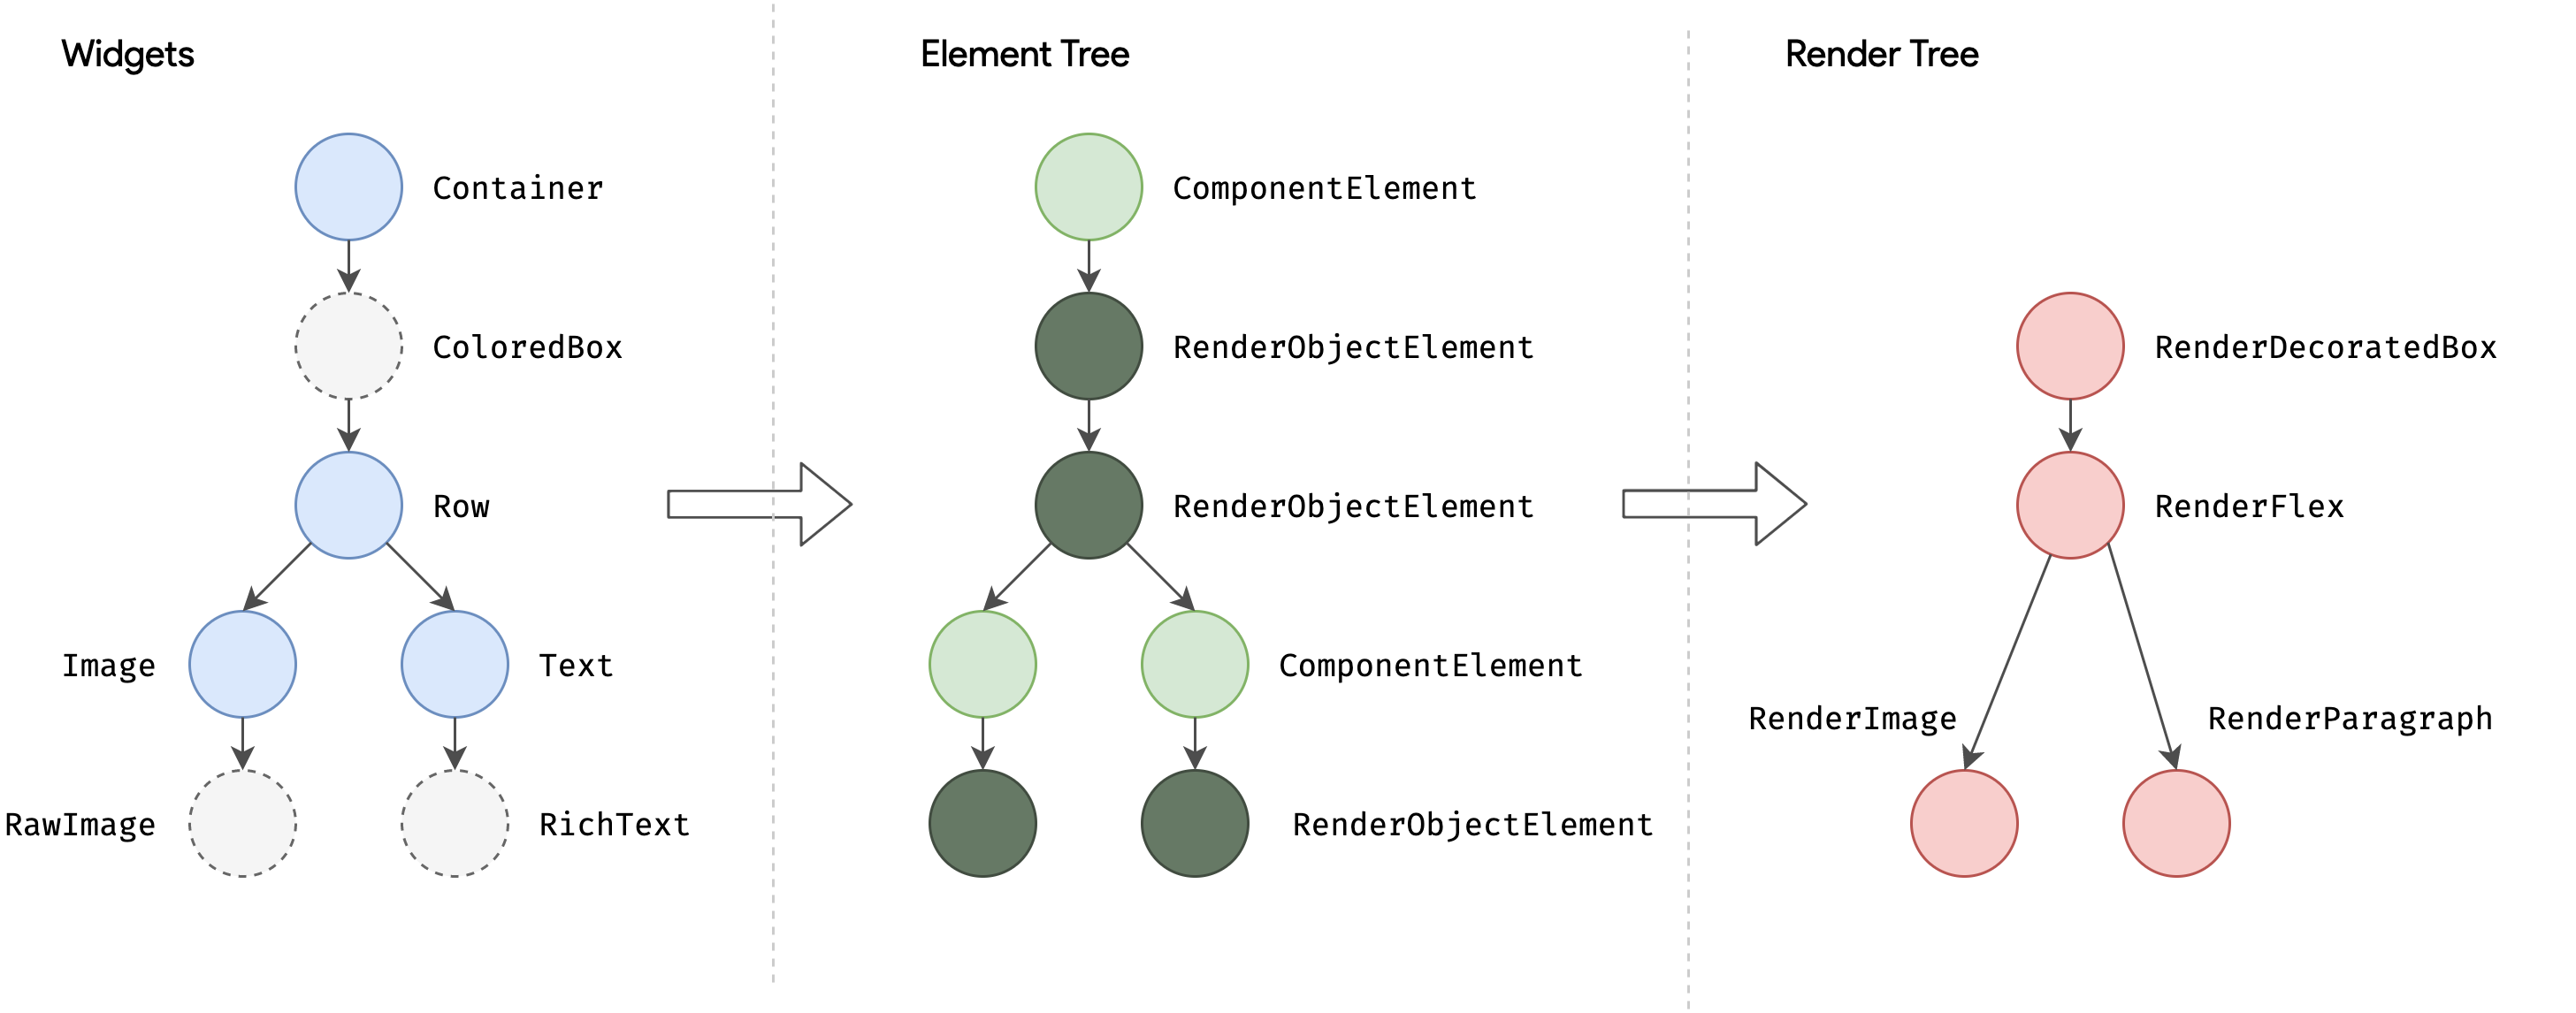
\includegraphics[width=1\textwidth]{flutter_trees.png}
  \caption{Flutter build proces}
  \label{fig:flutter_trees}
\end{figure}



\subsection{Compose Multiplatform}

Compose Multiplatform je framework sloužící k tvorbě uživatelských rozhraní použitelných na vícero platformách za 
jehož vývojem stojí společnost JetBrains. \cite{composeMultiplatform} Je založen na toolkitu zvaném Jetpack Compose, který je aktuálně 
doporučovaný k tvorbě nativních uživatelských rozhraních na platformě Android. \cite{jetpack}

Podporuje platformy jako Android, iOS (Alpha), Windows, MacOS, Linux a Web (experimentální). \cite{composeMultiplatform}

\medskip

\subsection*{Klíčové vlastnosti Compose Multiplatform}

\myparagraph{Deklarativní zápis UI} 
Používá deklarativní syntaxi pro popis uživatelského rozhraní. \cite{KMPUseCases}

\myparagraph{Jednotný kód pro různé platformy} 
Možnost sdílet kód pro Android, iOS, web i Desktop.

\myparagraph{Snadné migrace díky postupné integraci} 
Díky KMP je možné postupně implementovat jednotlivé částí aplikace i do již existujících aplikací s minimálním rizikem oproti
ostatním multiplatformním technologiím. \cite{KMP}

\myparagraph{Znovupoužitelnost Kotlin kódu} 
Díky KMP je možné použít některé části kódu z již existujících Android aplikací i na ostatních platformách.

\myparagraph{Programovací jazyk Kotlin} 
Frontendová i backendová část aplikace jsou psány v jazyce Kotlin pro bezproblémovou integraci se serverovou částí.

\myparagraph{Podpora od JetBrains}
Poskytuje stabilní podporu od vývojářského týmu JetBrains.

\subsection*{Architektura frameworku Compose Multiplatform}
Jelikož je framework Compose Multiplatform z velké části založen na frameworku Jetpack Compose, tak v této kapitole bude probírána
právě architektura toho frameworku, která bude doplněna o drobné rozdíly mezi těmito dvěma frameworky.

V porovnání s ostatními dříve zmíněnými frameworky slouží tento framework pouze k tvorbě multiplatformního UI a z toto důvodu je převážně 
používán s toolkitem Kotlin Multiplatform, který dané aplikaci poskytuje i multiplatformní aplikační logiku. Jelikož se jedná o základní 
komponentu bez které by Compose Multiplatform nevznikl, tak je tomuto toolkitu věnována celá kapitola. \ref{kmpSection}

Pro lepší ukázku toho z jakých částí se typická multiplatformní mobilní aplikace skládá slouží následující obrázek \ref{fig:composeIOS}.

\begin{figure}[H]
  \centering
  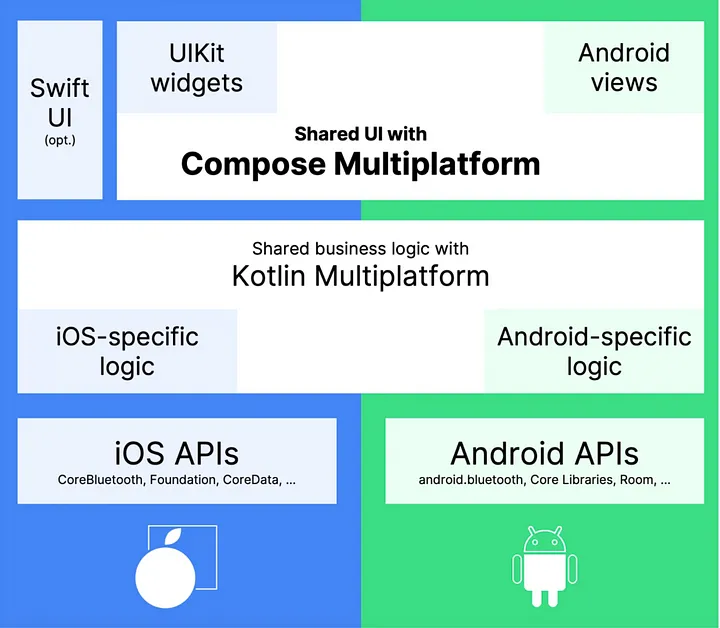
\includegraphics[width=.7\textwidth]{composeIOS.png}
  \caption{Compose Multiplatform iOS}
  \label{fig:composeIOS}
\end{figure}

Jak již bylo zmíněno tak 



Co se týče samotného UI kódu, tak ten se skládá z jednotlivým funkcí označených anotací \code{@Composable}, která k těle obsahuje další
\textit{Composable} funkce (viz výpis kódu \ref{lst:ComposeCode}) jako jsou například \code{Column} pro strukturování vnořených elementů do sloupce nebo \code{Text} pro výpis
textu na obrazovku. 


\begin{lstlisting}[caption={Popis UI widgetů pomocí jazyka Kotlin}, label={lst:ComposeCode}, language=Kotlin]
@Composable
fun MyComposable() {
    Column {
        Text("Hello")
        Text("World")
    }
}
\end{lstlisting}

Takto strukturovaný kód může být následně frameworkem vykreslen na obrazovku zařízení v těchto třech následujících fázích:

\myparagraph{Composition}
Během této fáze Jetpack Compose vytvoří stromovou strukturu reprezentující UI komponenty, které mají být vykresleny.\cite{jetpackPhases}

\myparagraph{Layout}
Během této fáze se jednotlivým komponentám určí na jaké pozice se dané komponenty vykreslí a jakou budou mít šířku a výšku.
Compose během této fáze prochází UI strom komponent tak, že nejprve měří své potomky pokud existují. Následně se na základě těchto
měření rozhodně o vlastní velikosti a nakonec umístí každého potomka relativně ke své pozici.\cite{jetpackPhases}

Díky použití tohoto algoritmu je k prostupu celého stromu zapotřebí navštívit každý uzel pouze jednou, což je výhodné jelikož
s přibývajícími uzly roste pouze lineárně. \cite{jetpackPhases}

\myparagraph{Drawing}
V rámci poslední fáze dochází s samotnému vykreslení komponent na obrazovku koncového zařízení. \cite{jetpackPhases}
Compose během této fáze znovu postupně prochází strom UI elementů od kořene až do listů a každý element tohoto stromu vykreslí sám sebe 
na pozici určenou během Layout fáze. \cite{jetpackPhases}

\subsubsection{Kotlin Multiplatform} \label{kmpSection}


%https://blog.jetbrains.com/kotlin/2023/11/kotlin-multiplatform-stable/#use-the-power-of-the-growing-kotlin-multiplatform-ecosystem

Kotlin Multiplatform je často základním kamenem pro tvorbu multiplatformních aplikací založených na Compose Multiplatform a to
z toho důvodu, že díky KMP je možné implementovat multiplatformní aplikační logiku, která může doplňovat multiplatformní UI 
poskytované frameworkem Compose Multiplatform. \cite{KMPUseCases} Důležitým rozdílem oproti ostatním multiplatformním frameworkům 
je právě ta možnost, kterou KMP případně Compose Multiplatform vývojářům poskytuje. 

Jelikož se jedná o SDK, tak umožňuje vývojářům implementovat multiplatformní funkcionality postupně, bez nutnosti implementovat 
v Kotlinu celé vrstvy aplikací. Díky tomu dává vývojářům možnost sdílet napříč platformami je ty části kódu, které mají největších
smysl implementovat pro veškeré platformy a zbylé části kódu psát v nativním jazyce pro danou platformu. \cite{KMP}
Lépe je tato skutečnost ilustrována na následujícím obrázku \ref{fig:KMP_vrstvy}, na kterém jsou vidět různé možnosti,
jakými může být KMP na daných platformách implementován.

\begin{figure}[H]
  \centering
  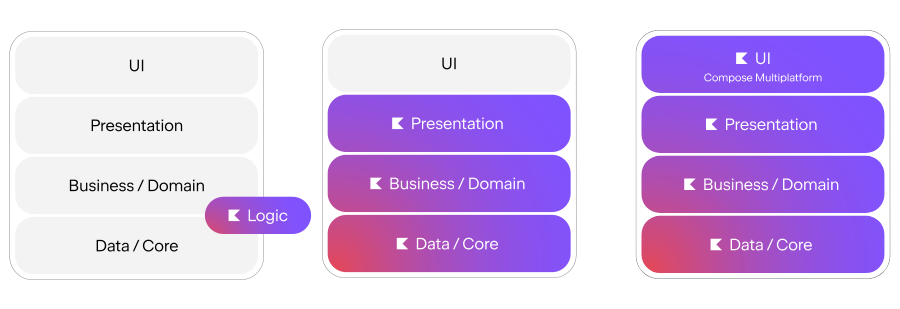
\includegraphics[width=1\textwidth]{KMP_vrstvy.png}
  \caption{Možnosti implementace KMP}
  \label{fig:KMP_vrstvy}
\end{figure}

Zároveň je tento obrázek možnou ukázkou toho, jak může probíhat migrace z již naimplementované nativní aplikace na aplikaci
multiplatformní. Nejprve je tedy možné implementovat jen malou část aplikační logiky pro víro platforem a postupem času přesouvat
do multiplatformní části aplikace například celé vrstvy starající se o prezentační, datovou nebo jinou aplikační logiku. \cite{KMPUseCases}

Aby ale k takové migraci mohlo dojít, tak je zapotřebí aby pro technologie používané v původní nativní aplikaci existovali multiplatformní
knihovny nebo alespoň jejich ekvivalent.

\subsubsection*{Multiplatformní knihovny}
Společnost JetBrains ve svém článku z konce roku 2023 zmiňuje, že existuje již přes 1500 KMP knihoven s tím, že ještě v roce 2020
jich bylo pouze několik málo desítek. \cite{KMPstable}

%Jeho hlavním úkolem je sdílení kódu na mobilních platformách. 
Právě počet a vyspělost těchto knihoven se podle společností, které již KMP používají jeví jako zatím jedna z nejslabších stránek KMP (viz kapitola \ref{kmpInPractise}).


\begin{figure}[H]
  \centering
  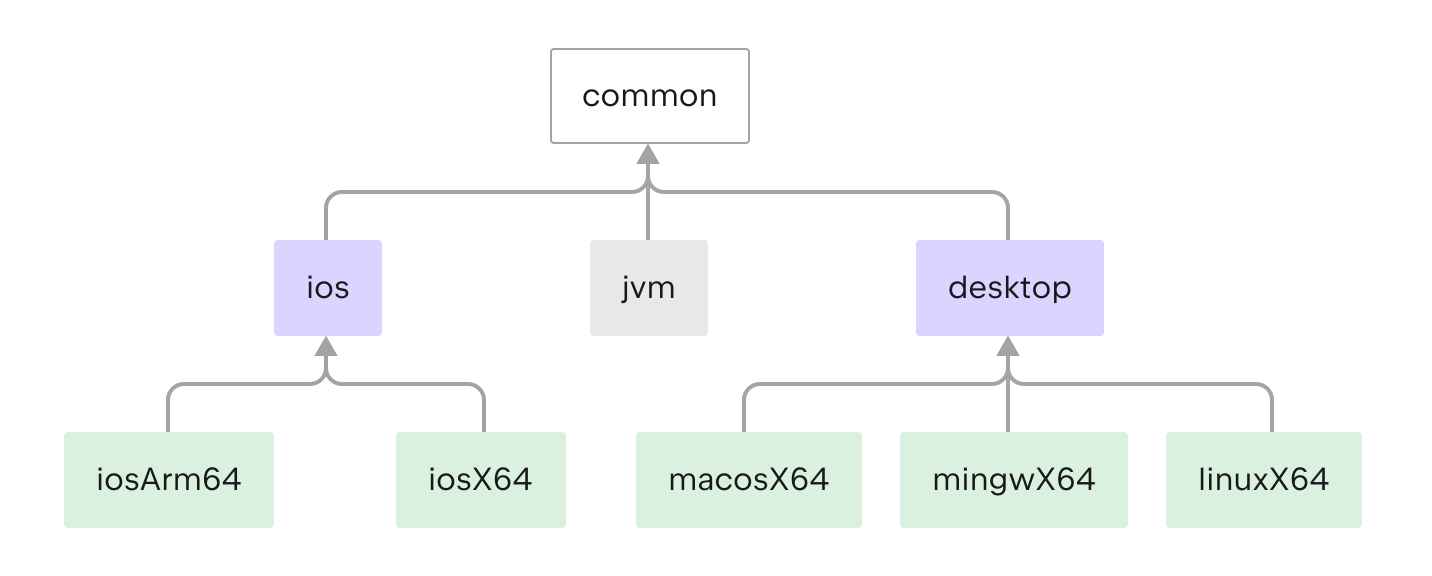
\includegraphics[width=1\textwidth]{kotlin-multiplatform-hierarchical-structure.png}
  \caption{Hierarchická struktura KMP}
  \label{fig:KMP_struktura}
\end{figure}

V případě, že žádná vhodná knihovna není k dispozici, tak je zde stále možnost čehož je možné docílit díky funkcionalitě jazyka Kotlina
zvané Expected a actual deklarace.

\subsubsection*{Expected a actual deklarace}\label{expectActual}
Deklarace \textit{expected} a \textit{actual} umožňují přistupovat k platformě specifickým API z Kotlin Multiplatform modulů. \cite{KMPExpectActual}
Nejprve je ve společné části potřeba vytvořit například třídu nebo funkci u které chceme aby její obsah byl implementován typicky pomocí
platformě specifických knihoven a tuto část v rámci společného modulu označit klíčovým slovem \code{expect}. \cite{KMPExpectActual} Její implementaci následně provést v rámci
platformě specifického kódu. Tato implementace musí být provedena pod stejným názvem a ve stejném balíku jako deklarace ve společném modulu
a musí být označena klíčovým slovem \code{actual}. \cite{KMPExpectActual}

Během kompilace pak Kotlin kompilátor každou deklaraci s klíčovým slovem \code{expect} sjednotí s příslušnou actual deklarací pro danou platformu
a vygeneruje z ní jednu deklaraci obsahující actual implementaci. \cite{KMPExpectActual}

\subsubsection*{Aktuální použití KMP v praxi} \label{kmpInPractise}
% Mezi další důvody patří taktéž lepší zastupitelnost jednotlivých členů týmu a to díky me

I přesto, že je KMP ve stabilní verzi teprve od listopadu 2023 \cite{KMPstable}, tak tuto technologii používá již několik světově 
známých firem v produkčním nasazení jako je například Forbes či McDonald's. Forbes uvádí, že právě díky KMP dokáží sdílet až 80 \%
aplikační logiky napříč platformami Android a iOS. \cite{KMPinForbes} 
Druhý ze jmenovaných McDonald's jako hlavní výhody uvádí jednodušší testování \cite{KMPinMcDonalds}

Naopak mezi největší výzvy, které obě společnosti ve svých souhrnech uvádějí patří adaptace na KMP prostředí (především iOS vývojářů) nebo
nedostatečné množství potřebných multiplatformních knihoven (případně jejich nedostatečná vyspělost). \cite{KMPinForbes} \cite{KMPinMcDonalds}

Pro porovnání 

\emph{"Od této doby jsme vyvinuli a v produkci provozujeme několik mobilních aplikací. Ze zkušenosti vidíme, že při jejich vývoji dokážeme sdílet cca 60–70 \% kódu na platformu. V případě vývoje na dvě platformy to znamená, že v součtu dokážeme ušetřit minimálně třetinu nákladů na vývoj, plus s tím související další náklady na věci typu testování (v tomto případě snížení až na polovinu)."}

\begin{figure}[H]
  \centering
  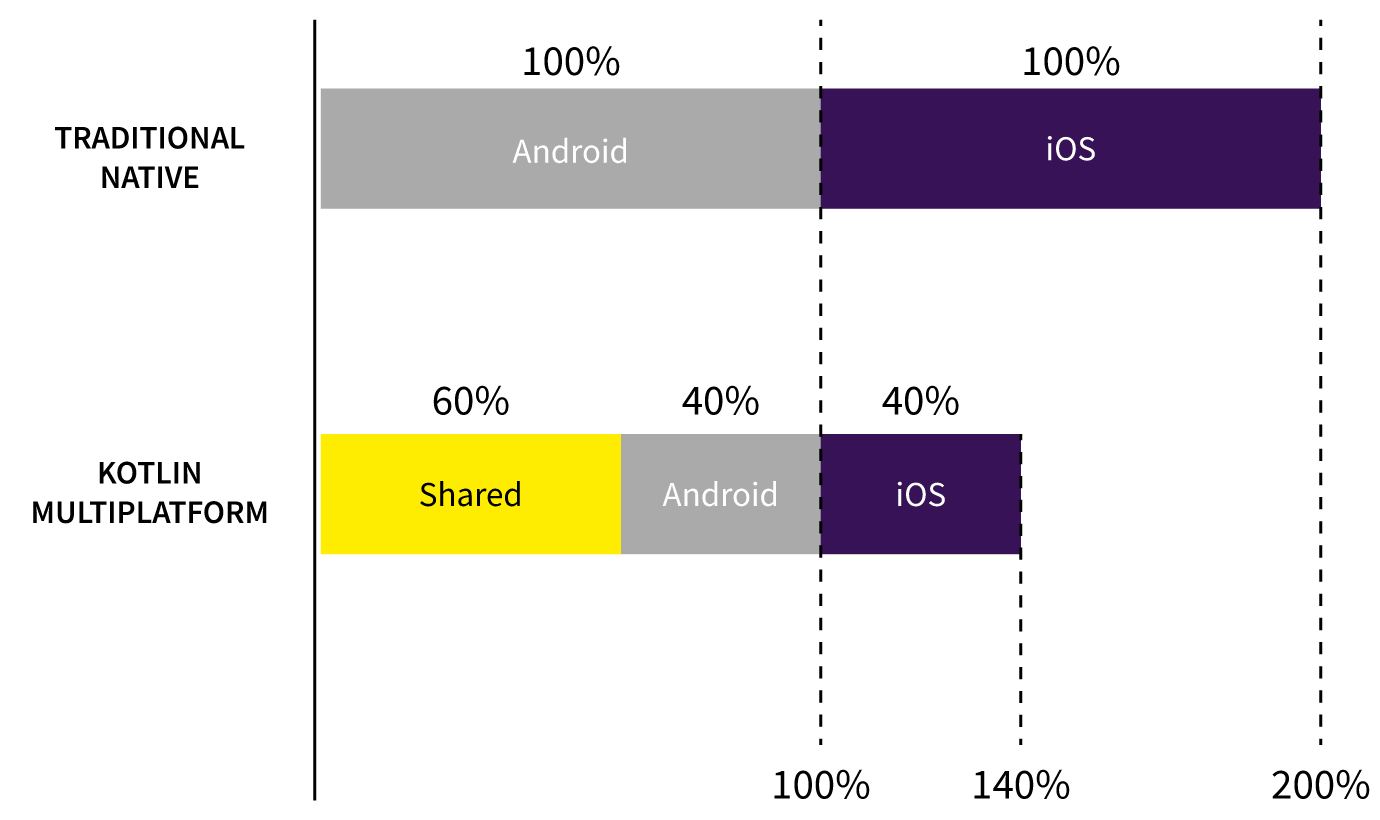
\includegraphics[width=.7\textwidth]{chart-KMP-vs-native.png}
  \caption{Množství kódu KMP vs native}
  \label{fig:KMP_vs_native}
\end{figure}

Pro upřesnění je ještě potřeba zmínit, že veškeré vyjmenované společnosti, využili pouze možnosti sdílení logiky a nepoužívají
tak sdílené UI pomocí Compose Multiplatform.

\section{Flutter vs React Native vs Compose Multiplatform}


\subsection{Porovnání výkonu}

Mezi klíčové parametry, kvůli kterým většina firem upřednostňuje vývoj nativních aplikací, patří jednoznačně výkon
nativních aplikací. Z toho důvodu se následující podkapitola věnuje právě porovnání výkonu a dalších parametrů s
nativními verzemi aplikací. 


\subsection*{Ukázková aplikace}

Pro porovnání důležitých parametrů byla pro test vytvořena jednoduchá aplikace, která obsahovala jednu obrazovku, 
načetla obrázky z veřejného API a zobrazila je v horizontálním seznamu. 
Na každý obrázek šlo kliknout a zobrazit jej přiblížený pod seznamem. 
Pro testování byly použity toolkity pro tvorbu nativního UI pro platformu Android (Jetpack Compose) a iOS (SwiftUI)
v porovnání s multiplatformními technologiemi Compose Multiplatform a Flutter.

Mezi hlavní testované parametry patřil čas nastartování testované aplikace a její velikost.

\myparagraph{Velikost aplikace}

Na obrázku \ref{fig:chart_app_sizes} je vidět, že velikost aplikace založené na Compose Multiplatform je identická
s velikostí nativní aplikace pro Android. Je tomu tak z toho důvodu, že výsledná aplikace pro Android neobsahuje kód 
pro jiné platformy. Kdežto u velikosti iOS aplikace je situace výrazně jiná. Samotná aplikace pro iOS je v porovnání
s její nativní aplikací o 23,1 MB větší. Tento rozdíl ve velikosti je způsoben především grafickou 2D knihovnou Skia,
která je na platformě Android dostupná, kdežto na platformě iOS ne a proto tam musí být spolu s aplikací dodána.

Zajímavé je následně porovnání s velikostí aplikace založené na frameworku Flutter, jelikož ta, stejně jako Compose
Multiplatform využívá knihovnu Skia, ale i přesto je o něco menší než Compose Multiplatform aplikace na platformě iOS.
Flutter Engine je součástí aplikace spolu s kódem Dart a zvětšuje velikost (asi 3–4 MB pro Android a 10 MB pro iOS).t

\begin{figure}[H]
  \centering
  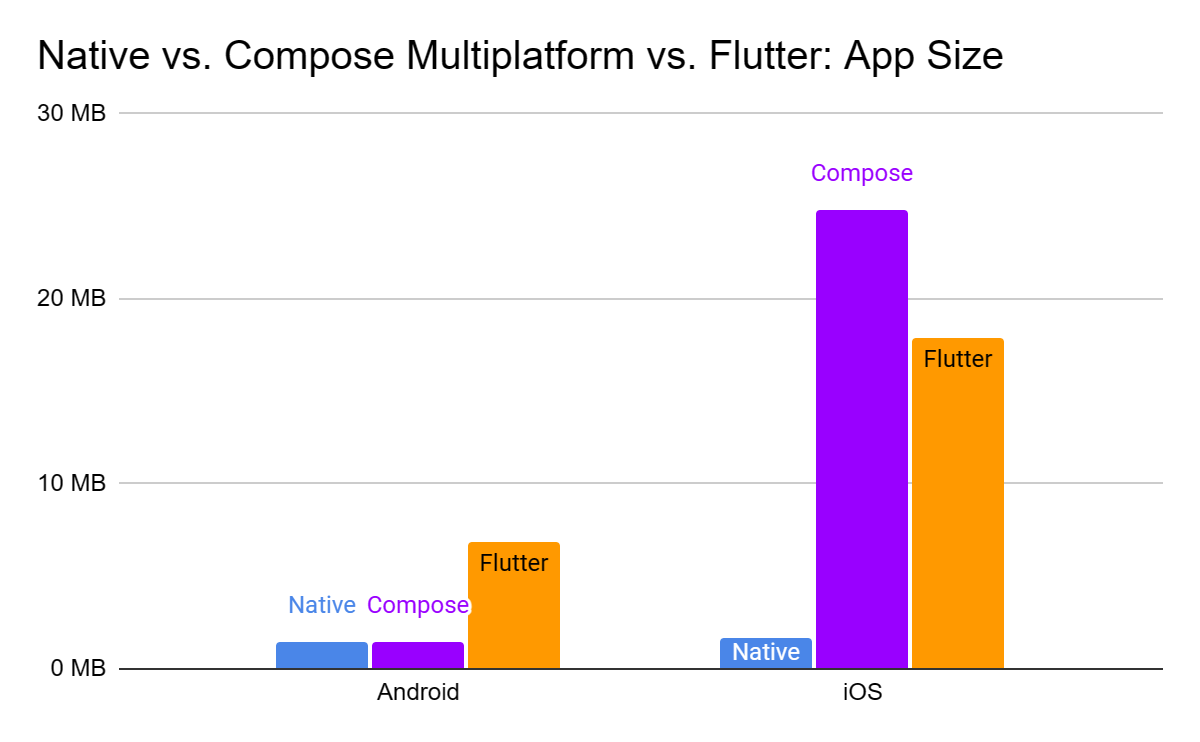
\includegraphics[width=.7\textwidth]{chart_app_sizes.png}
  \caption{APK/IPA size in megabytes}
  \label{fig:chart_app_sizes}
\end{figure}

\myparagraph{Rychlost spuštění aplikace}

Při porovnání rychlosti spuštění Compose Multiplatform aplikace na platformě Android není mezi rychlostmi téměř žádný
rozdíl stejně tak jako tomu při porovnání velikosti aplikací v předchozí kapitole. O něco delší dobu spuštění měla
aplikace napsaná pomocí frameworku Flutter, která se spouštěla v průměru o 221 ms déle než Compose Multiplatform aplikace. 
Toto zpomalení je s nejvyšší pravděpodobností způsobeno dobou spuštění Flutter Enginu, což by korespondovalo s oficiální
Flutter dokumentací. \cite{flutterPerformance}

U posledního porovnání na platformě iOS se doba spuštění aplikací založených na Compose Multiplatform a frameworku 
Flutter o tolik nelišila od nativní aplikace, což ukaje slibné použití těchto multiplatformních technologií v budoucnu.
% // TODO posledni cast porovnani

\begin{figure}[H]
  \centering
  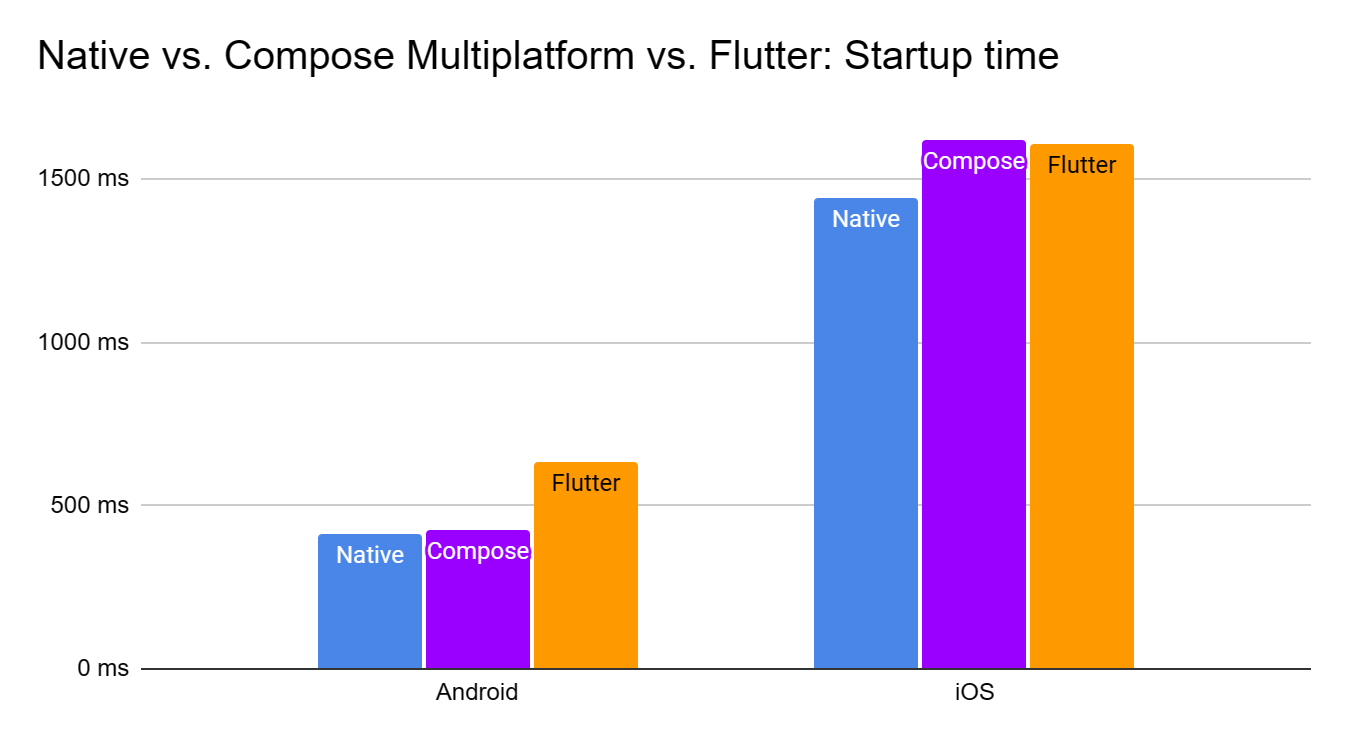
\includegraphics[width=.7\textwidth]{chart_startup_times.png}
  \caption{App startup time on a Pixel 4a and iPhone 12 Mini in milliseconds}
  \label{fig:chart_startup_times}
\end{figure}

\section{Náročnost implementace}
\section{Limitace Compose Multiplatform oproti nativnímu řešení} 
% to se tyka KMP ne compose Multiplatform
Jak již bylo zmíněno v kapitole KMP , tak jedním z největších problému multiplatformního vývoje je především nedostatečné množství knihoven. 

Co se týče UI, tak zde je situace díky možnosti využití Jetpack Compose o něco lepší. Většina omezení, která jsou
aktuálně spjata s UI se týká především plynulosti a nebo použití nativně vypadajících komponent na platformě iOS.
Ta v její nativní podobě používá styl zvaný Cupertino, který aktuálně není oficiálně podporován. Co se týče plynulosti UI
na platformě iOS, tak aktuálně se řeší problém s

Většina výše zmíněných problémů se již řeší a je zmíněna v Kotlin Multiplatform vývojářském plánu pro rok 2024. \cite{KMPRoaddMap} Konkrétně
se jedná o veškeré zmíněné o problémy kromě zařazení HarmonyOS mezi podporované platformy.% // todo 
V tomto plánu je mimo jiné uvedeno, že aktuální prioritu číslo jedna je dostání frameworku Compose Multiplatform na platformě iOS do verze Beta. \cite{KMPRoaddMap}

\chapter{Návrh}



\section{Výběr aplikace pro implementaci}
Základním požadavkem bylo vybrat takovou aplikaci, ve které by bylo možné použít velké množství různých komponent, 
které by bylo možné použít napříč různými platformami.
Mezi další požadavky patřilo zaměření se na kritické problémy související s multiplatformním vývojem. 
například využití funkcí, které jsou silně spjaty s hardwarem koncových zařízení jako třeba použití jednotné navigace

fotoaparátu, služeb lokalizace, 

Z těchto důvodů byla k implementaci vybrána aplikace sloužící pro občany měst či obcí, která kombinuje veškeré funkční
požadavky které plynou ze zadání.

Tato aplikace by sloužila občanům k získání informací o aktuálních novinkách, pořádaných akcích nebo jim umožňovala
zaplatit parkovné.

\section{Funkční požadavky}
Funkční požadavky definují konkrétní vlastnosti a chování aplikace, které zajistí, že bude aplikace pro občany měst či obcí 
užitečná, efektivní a snadno použitelná.

\myparagraph{Zobrazení novinek}
Možnost přidávat, editovat a mazat novinky a oznámení.
Zobrazení aktuálních novinek na domovské obrazovce aplikace.
Možnost filtrovat novinky podle kategorie nebo data.

\myparagraph{Zobrazení událostí}
Zobrazení kalendáře s událostmi, akcemi a důležitými daty.
Možnost procházet události v kalendáři dle data, místa nebo typu události.
Možnost přidávat nové události do kalendáře.
Možnost filtrovat události podle kategorie nebo data.

\myparagraph{Platební brána pro parkovné}
Možnost provádět platby parkovného prostřednictvím aplikace.
Zadání informací o vozidle, parkovacím místě a délce parkování.
Zobrazení historie plateb a možnost platit opakovaná parkování.

\myparagraph{Možnost vyhledání a kontaktování místních úřadů, policie nebo zdravotního střediska}
Zobrazení kontaktních informací a pracovní doby úřadů.
Možnost zaslat otázku, stížnost nebo žádost přímo prostřednictvím aplikace.
Správa uživatelského účtu:

\myparagraph{Možnost vytvoření a správa uživatelského účtu}
Přihlašování se pomocí e-mailu, telefonního čísla nebo sociálních sítí.
Ukládání osobních preferencí a nastavení aplikace.

\myparagraph{Navigace a mapy}
Integrace mapových služeb pro zobrazení umístění událostí a místních služeb.
Možnost vyhledávání tras a navigace v rámci města nebo obce.

\myparagraph{Podpora více jazyků}
Možnost nastavení jazyka aplikace dle uživatelských preferencí.
Zobrazení obsahu a textů v různých jazycích.

\myparagraph{Feedback a hodnocení}
Možnost zaslat zpětnou vazbu, hodnocení nebo recenzi na aplikaci.
Zpětná vazba od uživatelů a možnost sledovat spokojenost s aplikací.

\section{Use cases}

\myparagraph{Zobrazení aktuálních novinek} 
Uživatelé mohou prostřednictvím aplikace získat přístup k aktuálním novinkám, událostem a důležitým oznámením ze svého města nebo obce. Tato funkce umožní občanům zůstat informováni o dění ve svém okolí.

\myparagraph{Zobrazení aktuálních událostí} 
Aplikace poskytne uživatelům přehled o připravovaných akcích, událostech a kulturních aktivitách v jejich městě nebo obci. Uživatelé budou moci procházet kalendář akcí, filtrovat je podle svých zájmů a získat podrobnosti o jednotlivých událostech.

\myparagraph{Platba parkovného} 
Aplikace umožní uživatelům snadno a rychle zaplatit parkovné prostřednictvím svého mobilního zařízení. Uživatelé mohou zadat informace o svém vozidle, délce parkování a provedení platby online, což jim ušetří čas a nepohodlí spojené s hledáním parkovacího automatu nebo mincí.

\myparagraph{Kontakty na místní úřady} 
Aplikace může poskytovat možnost rychlého a snadného získání kontaktu na místní úřady nebo správními orgány. %Uživatelé budou moci prostřednictvím aplikace zasílat otázky, stížnosti nebo žádosti o pomoc a získávat odpovědi a podporu přímo ze svého mobilního zařízení.

\section{Návrh architektury}
Navržená architektura se z velké části drží architektonických principů shrnutých v Android dokumentaci. \cite{andDocArch}

\subsection*{Důležité principy}

\myparagraph{Separation of concerns}
Separation of concerns je princip návrhu softwaru, který popisuje důležitost oddělení různých funkcionalit do samostatných, dobře definovaných a izolovaných částí.
Hlavním cílem tohoto principu je zlepšit modularitu, udržitelnost, znovupoužitelnost a spravovatelnost kódu.

Princip oddělení zájmů rozděluje systém na jednotlivé komponenty nebo moduly, přičemž každý z nich se zabývá jednou konkrétní 
oblastí funkcionality. Každá část systému má jasně definované rozhraní, které umožňuje interakci s ostatními částmi. 
Tímto způsobem lze snadněji spravovat a udržovat kód, protože změny v jedné části systému nemusí mít nežádoucí dopady na ostatní části.

Příklady oddělení zájmů zahrnují oddělení prezentační vrstvy od logiky aplikace (Model-View-Controller), oddělení datového přístupu od 
podnikové logiky (Repository pattern), a oddělení různých vrstev aplikace (např. vrstva uživatelského rozhraní, aplikační logika, datová vrstva). 

\myparagraph{Unidirectional Data Flow}
Unidirectional Data Flow (jednosměrný tok dat) je architektonický vzor, který popisuje způsob, jakým data cestují skrz aplikaci. 
V tomto přístupu data proudí v jednom směru, což znamená, že existuje jasný a jednoznačný tok dat od zdroje až po jejich konečný cíl.
Takovýto přístup například umožňuje efektivní aktualizaci uživatelského rozhraní v reakci na změny dat a přispívá k jednoduchosti, 
předvídatelnosti a údržnosti softwarových aplikací.

\myparagraph{Single source of truth}
Princip Single Source of Truth (SSOT) je koncept v softwarovém inženýrství, který zdůrazňuje, že v aplikaci by měl existovat jediný 
zdroj dat, který obsahuje aktuální a spolehlivé informace. Tento zdroj dat je považován za „pravdivý“ a slouží jako jediný zdroj, 
ze kterého mohou ostatní části aplikace čerpat informace. Tím se zajišťuje konzistence dat napříč aplikací a minimalizuje se riziko 
konfliktů nebo chyb v datech.

Díky SSOT jsou data v aplikaci konzistentní a snadněji spravovatelná, protože všechny komponenty a moduly aplikace pracují se stejnými 
daty. To usnadňuje údržbu a vývoj aplikace, protože úpravy a aktualizace dat lze provádět centrálně. Z hlediska kódu přispívá tento
princip k jednoznačnosti a přehlednosti, protože vývojáři vědí, kde hledat relevantní data pro různé části aplikace.

Cílem tohoto konceptu je zlepšit konzistenci, přehlednost a údržbu aplikace a poskytnout spolehlivý zdroj dat pro všechny části aplikace.


\subsection{Vrstvy architektury}

Na základě těchto principů se ..., která uplatňuje výše zmíněné principy.
rozděluje architekturu do následujících třech vrstev:

\subsubsection*{UI vrstva}
UI vrstva se stará o zobrazení dat, která odpovídají aktuálnímu stavu a zároveň se 

\begin{figure}[H]
  \centering
  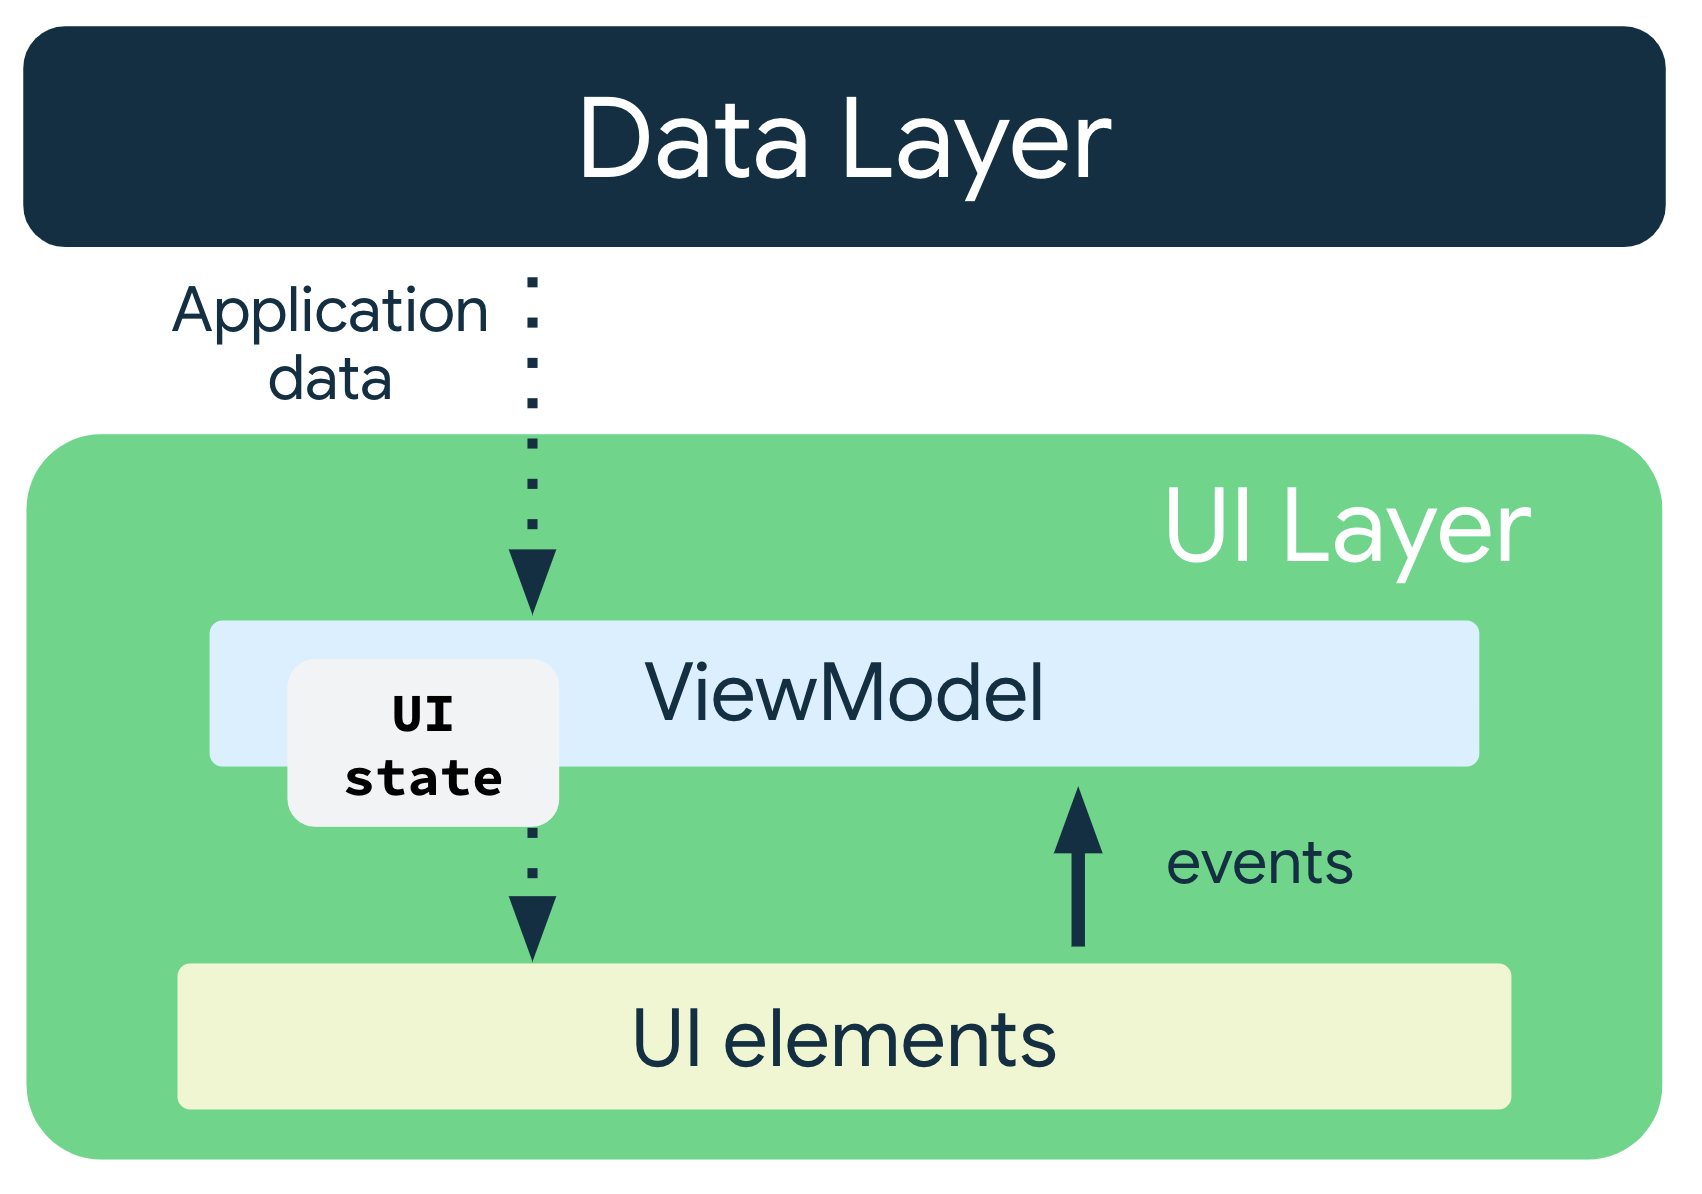
\includegraphics[width=.5\textwidth]{arch-ui-udf.png}
  \caption{Architektura UI vrstvy - UDF diagram}
  \label{fig:arch_ui_udf}
\end{figure}

\myparagraph{ViewModel}
Stará se logiku


Hlavní účel ViewModelu je uchovávat a spravovat data potřebná pro zobrazení na obrazovce, a to i při změnách konfigurace zařízení 
(například při otáčení obrazovky). ViewModel také poskytuje metody a události pro interakci s daty, jako je načítání dat ze zdroje, 
jejich aktualizace a předávání událostí od uživatele zpět do aplikace. Na základě těchto událostí například aktualizuje stav uživatelského
rozhraní.

\myparagraph{UI state} \label{UIStateParagraph}
UI state (stav uživatelského rozhraní) je koncept v softwarovém inženýrství, který popisuje aktuální stav a chování uživatelského 
rozhraní v daném okamžiku. Tento stav může zahrnovat různé informace, jako jsou aktuální hodnoty vstupních polí, stav vybraných prvků,
 aktuální zobrazené obrazovky nebo panely, stav animací a další.

UI state je důležitý pro udržování konzistence a interaktivity uživatelského rozhraní. Změny v UI stavu mohou být způsobeny uživatelskými
interakcemi, například kliknutím na tlačítko, zadáním textu do pole nebo rolováním seznamu, nebo mohou být vyvolány událostmi v aplikaci,
jako je získání dat ze serveru nebo změny v interním stavu aplikace.

Správa UI stavu je důležitou součástí vývoje aplikací s uživatelským rozhraním a může být implementována pomocí různých technik a nástrojů.
Důležité je udržovat UI stav v souladu s interním stavem aplikace a zajistit jeho konzistenci a správnou aktualizaci v reakci na uživatelské 
interakce a události v aplikaci.

\myparagraph{UI Elements}
Na základě poskytnuteho UI state zobrazují data reprezentující aktuální stav aplikace. Tento vztah je často d


UI elements neboli prvky uživatelského rozhraní jsou komponenty tvořící vizuální část aplikace a umožňují uživatelům interagovat s aplikací.
Tyto prvky zahrnují různé vizuální komponenty, jako jsou například tlačítka, textová pole, seznamy, obrázky, ikony, přepínače, posuvníky atd.

UI prvky jsou navrženy tak, aby poskytovaly uživatelům intuitivní způsob, jak manipulovat s aplikací a komunikovat s ní. Každý prvek má své 
vlastnosti, jako jsou velikost, barva, text, stav atd., Které lze nastavit a upravovat pomocí kódu. Tyto prvky jsou pak umístěny na obrazovce 
podle určeného rozvržení (layoutu), které určuje jejich pozici a vzájemné uspořádání.

UI prvky jsou základními stavebními bloky uživatelského rozhraní a hrají klíčovou roli při vytváření uživatelsky přívětivé a atraktivní aplikace. 
Jejich vhodné použití a umístění má vliv na celkový uživatelský zážitek a efektivnost aplikace.


\bigskip

Na následujícím výpisu kódu je vidět jakou strukturu bude mít následná implementace.

\begin{lstlisting}[caption={Popis UI widgetů pomocí jazyka Kotlin}, label={lst:ConsumeUIState}, language=Kotlin]
  @Composable
  fun LatestNewsScreen(
      viewModel: NewsViewModel = viewModel()
  ) {
      // Show UI elements based on the viewModel.uiState
  }
\end{lstlisting}

\subsection*{Doménová vrstva}
Doménová vrstva typicky obsahuje způsoby užití nicméně pro menší aplikace jako je tato může být vynechána. 

V tomto projektu doménovová vrstva zahrnuje deklarace výčtových typů, objektů pro datovou a modelou vrstvu a mapovací funkce pro pro převod
objeků datové vrstvy na objekty používané v prezentační vrstvě a naopak.

Doménová vrstva by měla být nezávislá na technických aspektech aplikace a měla by se zaměřovat pouze na reprezentaci a správu doménových
 konceptů a procesů. To zjednodušuje testování, údržbu a rozšíření aplikace a umožňuje snadnou změnu technologií nebo platformy bez 
 vlivu na doménovou logiku.

\subsection*{Datová vrstva}
Datová vrstva se stará o veškerá 
The data layer that contains the business logic of your app and exposes application data.


Datová vrstva je klíčovou součástí softwarových systémů, která se zabývá persistencí dat a komunikací s datovými úložišti, jako jsou
 databáze, soubory nebo vzdálené API. Jejím hlavním úkolem je poskytovat rozhraní mezi doménovou logikou aplikace a datovými zdroji, 
 aby bylo možné ukládat, načítat, aktualizovat a mazat data podle potřeby.



\begin{figure}[H]
  \centering
  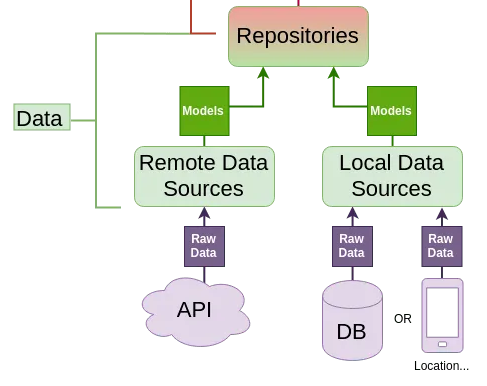
\includegraphics[width=.5\textwidth]{data_layer_diagram.png}
  \caption{Architektura datové vrstvy}
  \label{fig:arch_data_layer}23
\end{figure}

% \begin{figure}[H]
%   \centering
%   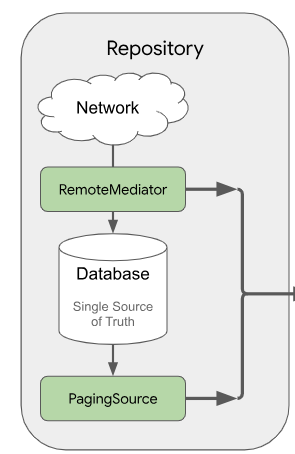
\includegraphics[width=.3\textwidth]{data_layer_diagram_principle.png}
%   \caption{Architektura datové vrstvy}
%   \label{fig:arch_data_layer_principle}
% \end{figure}

Mezi důležité prvky datové vrstvy patří:

\myparagraph{DAOs}
DAOs jsou zodpovědné za přímý přístup k datovým úložištím a provádění operací jako čtení, zápis, aktualizace a mazání dat. Tyto objekty 
poskytují abstrakci nad konkrétními technologiemi datových úložišť a umožňují snadnou změnu úložišť bez vlivu na ostatní části aplikace.

\myparagraph{DTOs}
DTOs jsou objekty používané k přenosu dat mezi vrstvami aplikace. Tyto objekty slouží k přenosu dat mezi datovou vrstvou a doménovou 
vrstvou a často mapují datové entity na jednodušší objekty nebo struktury pro snadnější manipulaci.

\myparagraph{Datové entity}
Datové entity představují strukturu a schéma dat uložených v databázi nebo jiném datovém úložišti. Tyto entity obvykle přímo odrážejí
strukturu tabulek v relační databázi nebo dokumentů v NoSQL databázi a poskytují model, se kterým mohou pracovat ostatní vrstvy aplikace.

\myparagraph{Datová úložiště}
Datové úložiště jsou fyzická místa, kde jsou data uložena. Mohou to být relační databáze, NoSQL databáze, soubory na disku nebo externí API. 
Datová vrstva zajišťuje, aby bylo možné efektivně pracovat s těmito úložišti a aby byla data bezpečně uložena a získána.

\bigskip

Tyto vrstvy jsou spolu propojeny následujícím způsobem.

\begin{figure}[H]
  \centering
  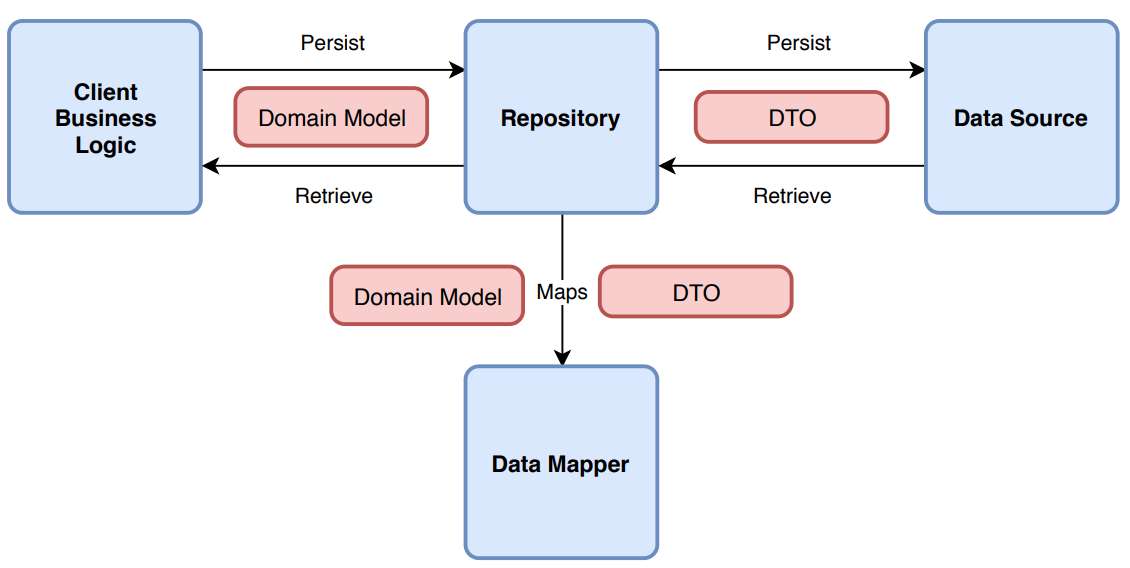
\includegraphics[width=.8\textwidth]{arch_diagram.png}
  \caption{Provázanost jednotlivých částí datové vrstvy}
  \label{fig:arch_diagram}
\end{figure}

\bigskip

Po shrnutí dosavadně zmíněních poznatků týkajících se architektury aplikace byly jednotlivé vrstvy převedeny do jednotlivých balíků s následující
strukturou:

\dirtree{%
.1 data\DTcomment{datová vrstva}.
  .2 model\DTcomment{}.
  .2 repository.
.1 ui\DTcomment{prezentační vrstva}.
  .2 composables\DTcomment{}.
  .2 screens\DTcomment{}.
    .3 HomeScreen\DTcomment{}.
}
\bigskip



% \dirtree{%
%         .1 src \DTcomment{}.
%           .2 androidMain \DTcomment{}.
%           .2 commonMain \DTcomment{je pro kód sdílený mezi všemi platformami}.
%             .3 kotlin \DTcomment{}.
%               .4 data\DTcomment{datová vrstva}.
% 		            .5 model\DTcomment{}.
% 		            .5 repository.
% 		          .4 ui\DTcomment{prezentační vrstva}.
% 		            .5 composables\DTcomment{}.
% 		            .5 screens\DTcomment{}.
% 		              .6 HomeScreen\DTcomment{}.
%             .3 resourses \DTcomment{}.
%           .2 desktop Main \DTcomment{}.
% 	}


% \begin{figure}[H]
%   \centering
%   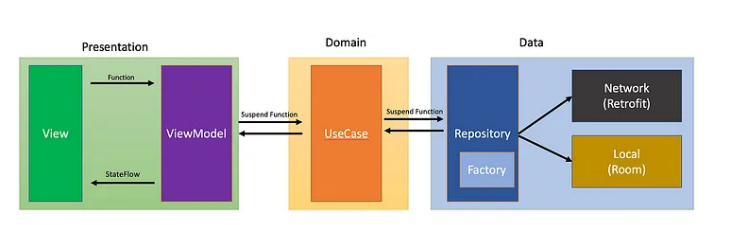
\includegraphics[width=1\textwidth]{mvvm.png}
%   \caption{MVVM with Clean Architecture}
%   \label{fig:mvvm}
% \end{figure}

\section{Návrh wireframes}
Navržené drátové modely byly vytvořeny na základě funkčních požadavků a to tak, aby nejdůležitější a nejčastěji používané funkce byly 
umístněny na domovkou obrazovku. A zbylé méně podstatbé nebo prostorově náročnější byli umístěny na sekundární obrazovky.

Zároveň byla snaha o 

Na základně...byla pro události vybrána možnost zobrazení jednotlivých událostí v LazyRow a to především z důvodu, že 
akce poutají především svým vizuálním největší část informace he uživateli předána právě pomocí titulního obrázku, názvu
a času konání.

Oproti tomu pro seznam novinek byl vybrán takzvaný LazyColum, který lépe umožňuje vyžít celou šíři obrazovky pro často delší
titulek a text události.

Obě tyto komponent navíc nabízí postupné načítání jejich obsahu, což nezpomaluje načítání obsahu v případně většího množství novinek
nebo událostí.

Mezi další UI prvky na domovské obrazovce patří tlačítka v její horní části, která uživateli umožňují proklik na YouTube kanál města,
nahlášení závady, zobrazení uředních hodin a kontaktů 

\begin{figure}[H]
    \minipage{0.38\textwidth}
      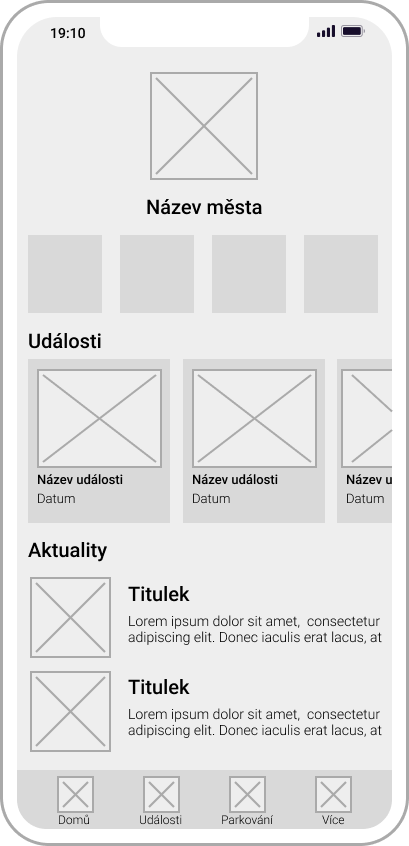
\includegraphics[width=\linewidth]{home_wireframe.png}
      \caption{Domovská obrazovka}\label{fig:screen1}
    \endminipage\hfill
    \minipage{0.4\textwidth}
      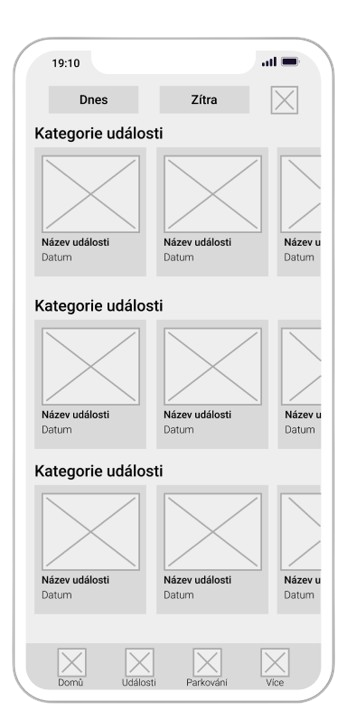
\includegraphics[width=\linewidth]{events_wireframe.png}
      \caption{Obrazovka akcí}\label{fig:screen2}
    \endminipage\hfill
\end{figure}

\begin{figure}[H]
    \minipage{0.4\textwidth}
    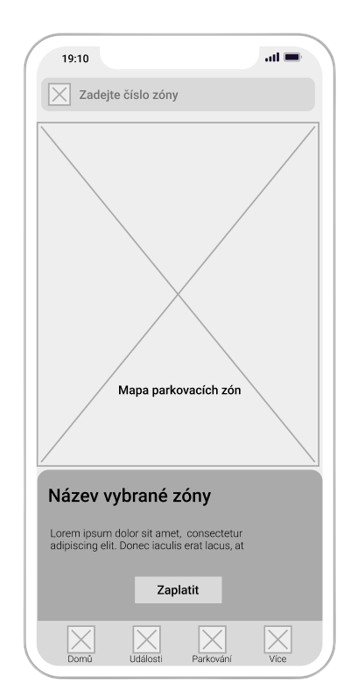
\includegraphics[width=\linewidth]{parking_wireframe.png}
    \caption{Screen 3}\label{fig:screen3}
  \endminipage\hfill
  \minipage{0.4\textwidth}
    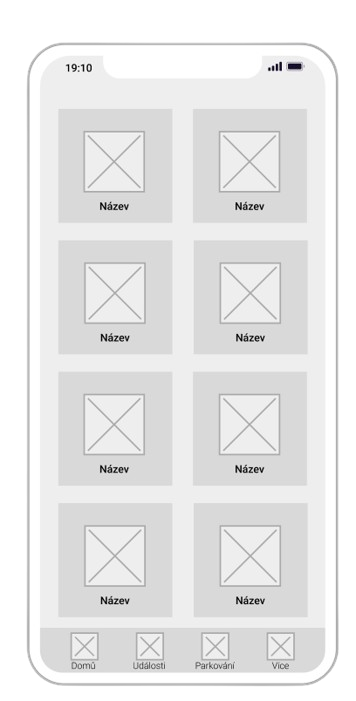
\includegraphics[width=\linewidth]{more_wireframe.png}
    \caption{Screen 4}\label{fig:screen4}
  \endminipage\hfill
\end{figure}

\section{Návrh grafické podoby UI}
Pro návrh grafické podoby UI byly použity prvky používané  barvy používané v rámci 
mockup

\begin{figure}[H]
    \minipage{0.4\textwidth}
      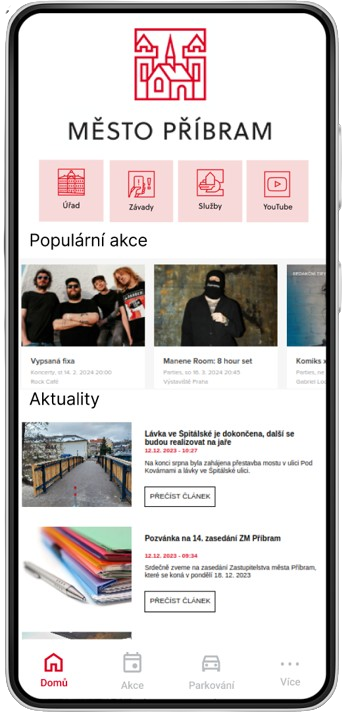
\includegraphics[width=\linewidth]{screen1.png}
      \caption{Domovská obrazovka}\label{fig:screen1}
    \endminipage\hfill
    \minipage{0.4\textwidth}
      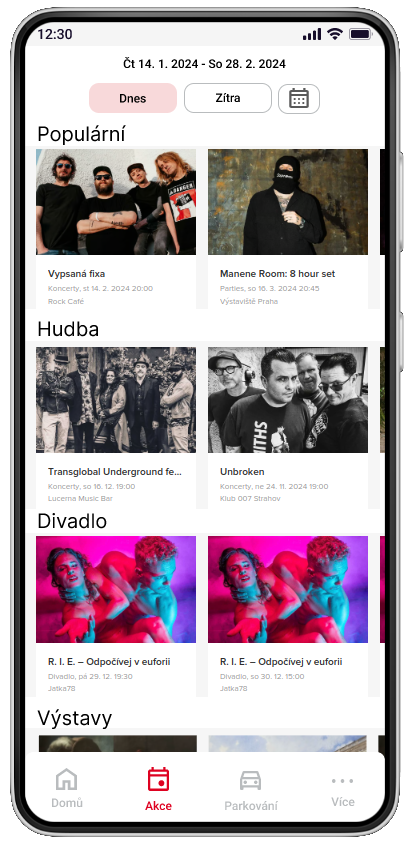
\includegraphics[width=\linewidth]{screen2.png}
      \caption{Obrazovka akcí}\label{fig:screen2}
    \endminipage\hfill
\end{figure}

\begin{figure}[H]
    \minipage{0.4\textwidth}
    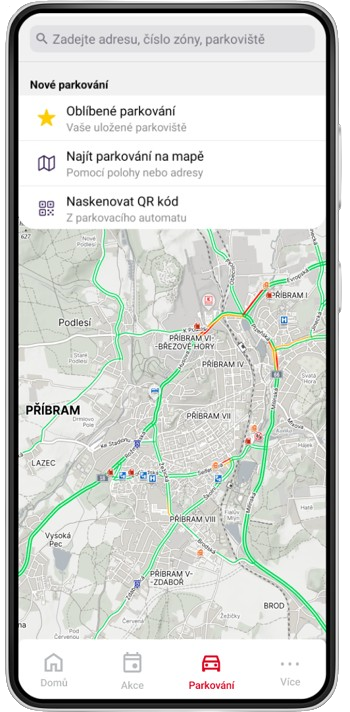
\includegraphics[width=\linewidth]{screen3.png}
    \caption{Screen 3}\label{fig:screen3}
  \endminipage\hfill
  \minipage{0.4\textwidth}
    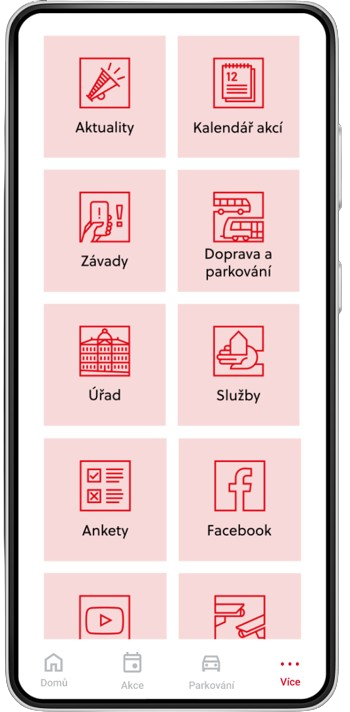
\includegraphics[width=\linewidth]{screen4.png}
    \caption{Screen 4}\label{fig:screen4}
  \endminipage\hfill
\end{figure}

\chapter{Implementace}
Stejně tak jako v případě vývoje Android aplikací, tak k sestavování multipaltformích aplikací založených na Compose Multiplatform 
se používá nástroj zvaný Gradle.  

\section{Gradle}
Gradle je open-source nástroj pro automatizaci sestavení a správu závislostí při vývoji softwaru. Je to nástroj pro automatizaci sestavení 
podobný Antu nebo Mavenu, který byl vyvinut pro zjednodušení procesu sestavení a nasazení softwaru.

Gradle používá deklarativní doménově specifické jazyky (DSL), díky kterým umožňuje definovat sestavení a konfiguraci projektu pomocí srozumitelné
a flexibilní syntaxe. Od verze 3.0 z roku 2016 je možné psát Gradle skripty v jazyce Kotlin DSL a od roku 2023 je Kotlin DSL primarním jazykem 
pro jejich zápis. To umožňuje vývojářům snadno konfigurovat sestavení a spravovat závislosti na knihovnách a modulech v jazyku se stejnou
syntaxí jako je používána pro ostatní části projektu.

%K vytvoření projektu založeném na Compose Multiplatform je doporučeno využití právě totoho sestavovacího nástoroje. 

K tomu aby bylo možné Compose Multiplatform v projektu použít, je zapotřebí do projektového souboru \code{build.gradle.kts} přidat Compose 
Multiplatform plugin (viz výpis kódu \ref{lst:ComposePlugin}).

\begin{lstlisting}[caption={Integrace Compose Multiplatform pluginu do sestavovacího scriptu}, label={lst:ComposePlugin}, language=Kotlin]
plugins {
  id("org.jetbrains.compose") version "1.6.0"
}
\end{lstlisting}
Dále je zapotřebí vybrat platformy pro které má být aplikace určena a podle nich vytvořit příslušné balíčky viz kapitola \ref{}.
Podle těchto balíčků se následně v příslušném \code{build.gradle.kts} vytvořit takzvané \code{sourceSets}, díky kterým je možné
pro každou platformu (balíček) implementovat platformě specifické závislosti. Tyto závislosti se následně vkládají do příslušných
sourceSets podle toho zdali se jedna o multiplatformní (commonMain) nebo nativní závislost (androidMain, iosMain, atd.).

Pro ukázky jak taková multiplatformní závislost může vypadat slouží ukázka kódu \ref{lst:LibIntegration}, díky které je do projektu
přidána knihovna umožnující implementaci multiplatformní navigace.

\begin{lstlisting}[caption={Lib integration}, label={lst:LibIntegration}, language=Kotlin]
sourceSets {
  commonMain.dependencies {
    implementation(libs.voyager.navigator)
    ...
  }
}
\end{lstlisting}

Dále je potřeba do spouštěcích souborů každé platformy integrovat multiplatformní část aplikace, která může být do nativního kódu přidána
například pomocí \textit{Composable} funkce, která je napsána v rámci sdílené části aplikace.

Ve výpisu kódu \ref{lst:SharedIntegration} je touto funkcí funkce \code{App()}, která je volána z nativního Android kódu a stará se
o deklaraci veškerého multiplatformního UI.

\begin{lstlisting}[caption={Lib integration}, label={lst:SharedIntegration}, language=Kotlin]
class MainActivity : ComponentActivity() {

  override fun onCreate(savedInstanceState: Bundle?) {
      super.onCreate(savedInstanceState)

      setContent {
          App()
      }
  }
}
\end{lstlisting}

Stejným způsobem je potřeba integrovat tuto funkci i do ostatních spouštěcích souborů.


Jelikož časem projekt obsahuje je vhodné pro správu verzí použít takzvaný version katalog. 

\myparagraph{Gradle version catalog}
Gradle version catalog je obyčejní soubor ve formátu TOML, který umožňuje snadněji přidávat a spravovat závislosti a pluginy ve celém projektu. 
Místo ručního přidávání závislostí a pluginů do každého modulu zvlášť je možné shromáždit veškeré závisloti v tomto souboru a zadefinovat rovněž
verzi, která má být pro tento modul použita napříč celým projektem. 

Příklad toho jak mohou být dříve zmíněné závislosti přepsány do version
katalogu je uveden ve výpisu kódu \ref{lst:VersionCalalog}.

\begin{lstlisting}[caption={Version katalog}, label={lst:VersionCalalog}, language=Kotlin]
[versions]
compose-plugin = "1.6.0"
voyagerVersion = "1.0.0"

[libraries]
voyager-navigator = { module = "cafe.adriel.voyager:voyager-navigator", 
                      version.ref = "voyagerVersion" }
[plugins]
jetbrainsCompose = { id = "org.jetbrains.compose",
                     version.ref = "compose-plugin" }

\end{lstlisting}

\section{Handling stavu}
Tato kapitola slouží k příblížení toho jak takzvaný \textit{UI State}, kterému byl věnován paragraf \ref{UIStateParagraph} v 
kapitole \textit{Vrstvy architektury} je implemementován v rámci ukázkové aplikace.

Z pohledu UI se jedná o důležitou část aplikace o jejíž aktualizaci se stará již smíněný ViewModel \ref{} neboli ScreenModel v rámci
implementované aplikace. 
Pro uchování stavu jednotlivých obrazek byl 



Jak již byl zmíněno v kapitole tak konkrétně v paragrafu zabívajícím se prací s UI stavy 

\section{Tvorba UI obecně}
\subsection{Navigace}
Navigace je klíčovou součástí moderních aplikací uživatelského rozhraní, která uživatelům umožňuje pohybovat se mezi různými obrazovkami či 
částmi aplikace. Hlavním cílem navigace je poskytnout uživatelům intuitivní a plynulý způsob průchodu obsahu a provádění akcí v aplikaci. 

Aktuálně však komponenta navizage ze sady knihoven Jetpack Compose není k dispozici a proto je potřeba zvolit nějakou alternativu poskytovanou
třetí stranou. \cite{composeNav} Výčet aktuálně doporučených knihoven pro implementaci multipaltformí navigace je uveden v oficiálních Kotlin 
multiplatform dokumentaci a zahrnuje navigace Voyager, Decompose nebo Appyx. K implemnaci byl po zvážení nakonec vybrána navigace Voyager a 
to především díky přehledné dokumentaci, intuitivní implementaci a jednoduchému principu navigace založeném na zásobníku, který pro aktuálně
implementovanou aplikaci plně dostačuje.

V budoucu by však měla být dostupná, ale do té doby je potřeba vybrat z alternativních knihoven.



%\section{Navigace a lokalizace v implementaci}
\subsection{Implementace design systému}
Design systém je sada předem definovaných pravidel, komponent, standardů a návrhových principů, které slouží k vytváření a udržování 
konzistentního a jednotného vizuálního stylu v rámci celé aplikce. Takový systém tak zahrnuje různé prvky jako jsou barvy, typografie, ikony,
layouty a komponenty uživatelského rozhraní a umožňuje vývojářům a designérům efektivně spolupracovat a vytvářet aplikace s jednotným 
vzhledem. 

V rámci vybraného města Příbrami není tento systém nikde expliciteně zadefinovaný a proto byl odvozen od designu webových stránek města.

Zároveň byl zkobinovaný s aktuálně nejnovějším design systémem od společnosti Google zvaným Material 3.


loading


\subsubsection{Barvy}
Barvy byly zvoleny na základě vizuálního stylu města, které Příbram využívá při všech prezentačních příležitostech.

a následně byly zadefinovánovány:

\begin{lstlisting}[caption={Zadefinování barev}, label={lst:ComposeCode}, language=Kotlin]
  val md_theme_light_primary = Color(0xFFBC004C)
  val md_theme_light_onPrimary = Color(0xFFFFFFFF)
  val md_theme_light_primaryContainer = Color(0xFFFFD9DE)
  val md_theme_light_onPrimaryContainer = Color(0xFF400015)
  ...

  val md_theme_dark_primary = Color(0xFFFFB2BE)
  val md_theme_dark_onPrimary = Color(0xFF660026)
  val md_theme_dark_primaryContainer = Color(0xFF900039)
  val md_theme_dark_onPrimaryContainer = Color(0xFFFFD9DE)
  ...
\end{lstlisting}

Takto zadefinované barvy je následně možné použít napříč aplikací k obarvení tlačítek, textů atd.

Mimojiné jsou taktéž použity pro definování barevných motivů, které se definují následujícím způsobem:

\begin{lstlisting}[caption={Definice barevných motivů}, label={lst:ComposeCode}, language=Kotlin]
  private val LightColors = lightColorScheme(
    primary = md_theme_light_primary,
    onPrimary = md_theme_light_onPrimary,
    primaryContainer = md_theme_light_primaryContainer,
    onPrimaryContainer = md_theme_light_onPrimaryContainer,
    secondary = md_theme_light_secondary,
    ...
  )

  private val DarkColors = darkColorScheme(
    primary = md_theme_dark_primary,
    onPrimary = md_theme_dark_onPrimary,
    primaryContainer = md_theme_dark_primaryContainer,
    ...
  )
\end{lstlisting}

Díky takto zadefinovaným barvám je následně možné obarvit jednotlivé komponenty aplikac podle zvoleného režimu.

\begin{lstlisting}[caption={Definice barevných motivů}, label={lst:colorsDef}, language=Kotlin]
  @Composable
  fun AppTheme(
    useDarkTheme: Boolean = isSystemInDarkTheme(),
    content: @Composable() () -> Unit
  ) {
    val colors = if (!useDarkTheme) {
      LightColors
    } else {
      DarkColors
    }
  
    MaterialTheme(
      colorScheme = colors,
      content = content
    )
  }
\end{lstlisting}

\subsubsection{Typografie}
je používána k definování stylu písma. Využívá k tomu styly definované Material designem. ten definuje celkem 15 stylů písma,
kde každé z nich má definovaný způsob použití. \cite{material3} Jelikož se jedná o výchozí styly písma, tak lze k těmto stylům přistupovat přes
Composable funkci \code{MaterialTheme} popsanou v kódu \ref{lst:colorsDef} aniž by se parametr \code{typography} musel explicitně
uvádět.

\begin{lstlisting}[caption={Ukázka použití stylu písma}, label={lst:typographyExample}, language=Kotlin]
  Text(
    text = news.title,
    style = MaterialTheme.typography.headlineMedium
  )
\end{lstlisting}

Výsledek základní ukázky takto navrženého systému je na obrázku \ref{fig:design_system}

\begin{figure}[H]
  \centering
  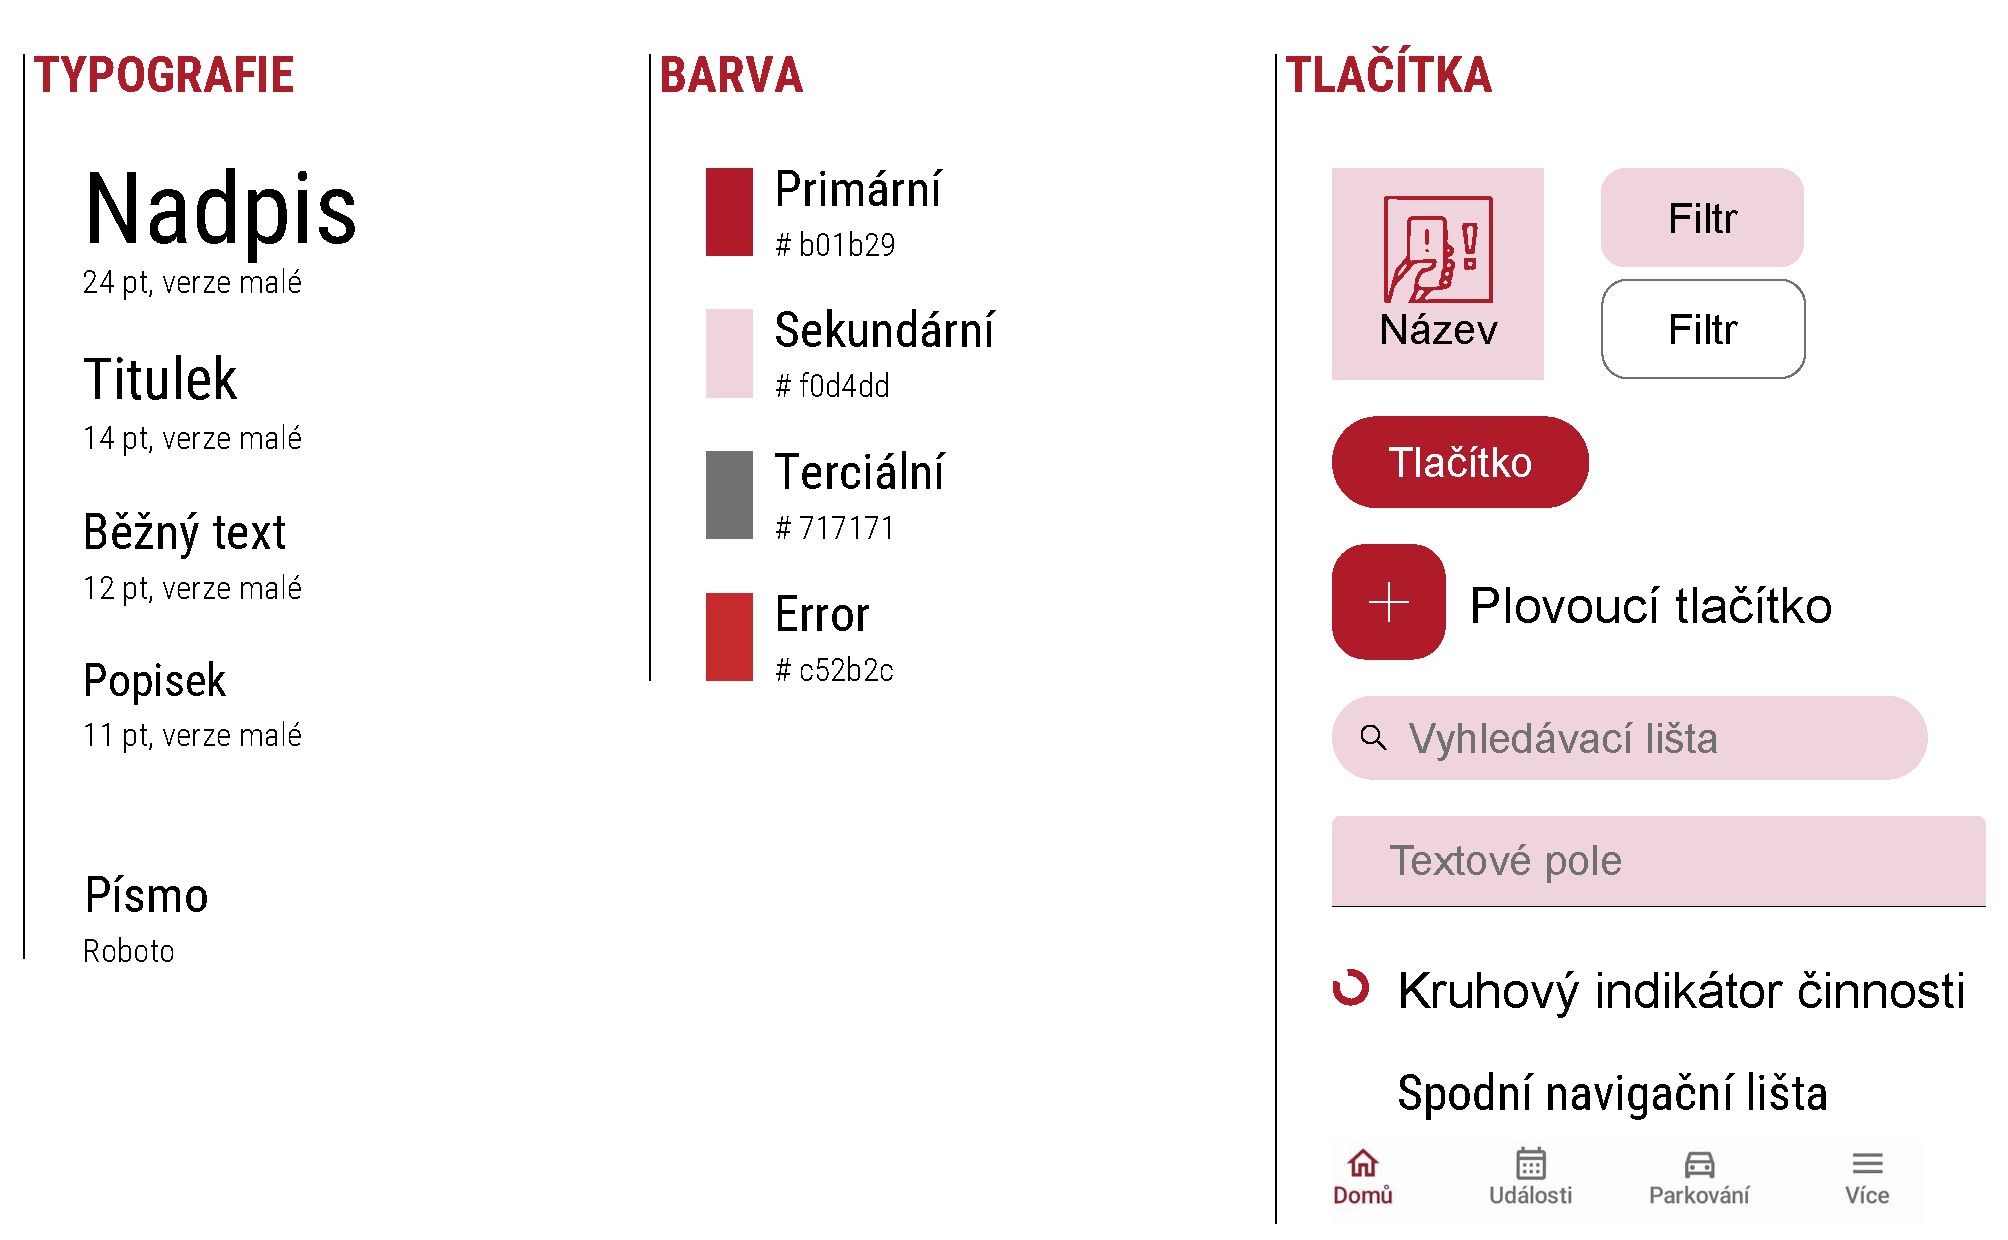
\includegraphics[width=.99\textwidth]{design_system.jpg}
  \caption{Vytvořený design systém}
  \label{fig:design_system}
\end{figure}

\section{Technologie - jen multiplatformní? }
Následující podkapitola je věnována konkrétním technologiím, které byli pro tvorku komponent z předchozí kapitoli použity.

\subsection{Kotlin}
\subsection{Coroutines}
\subsection{Ktor}
\subsection{Voyager}
Voyager je multiplatformní navigační knihovna, která umožňuje navigovat mezi různými obrazovkami a destinacemi v multiplatformních mobilních
 aplikacích. \cite{voyager} Jeho hlavním cílem je poskytnout jednotné rozhraní pro navigaci v různých mobilních platformách, jako jsou Android a iOS, a 
 zároveň maximalizovat sdílený kód a snižovat duplikaci kódu.

 V rámci implementované aplikace byla Voyager navigace použita k implementaci základní navigace mezi jedlotlivými obrazovkami.
 Příkladem takové navigace je přechod mezi 
 
 takzvané \textit{Tab navigation} čili navigace aplikací
 pomocí záložek ve spodní části displaye. 




\subsection{Koin}
Koin je moderní knihovna pro správu závislostí v aplikacích napsaných v jazyce Kotlin. Jedná se o lehkou a snadno použitelnou alternativu 
k jiným známým knihovnám, jako je například Dagger. Koin se zaměřuje na jednoduchost použití a minimalismus, což usnadňuje vývoj aplikací 
a zároveň zlepšuje čitelnost a údržbu kódu.

Hlavním principem Koinu je deklarativní přístup k definici závislostí pomocí tzv. modulů. V modulu se specifikují všechny závislosti a 
jejich vytváření, a to pomocí jednoduchých funkcí nebo tzv. singletons. Tento přístup umožňuje snadnou konfiguraci závislostí a poskytuje
 vývojářům transparentní pohled na strukturu aplikace.

\bigskip

V rámci této aplikace byl Koin použit například pro vložení databázového ovladače za pomocí expect actual deklarace \ref{expectActual}.
Využití tohoto zápisu bylo vhodné použít především díky tomu, že převážná většitna databázové logiky je napsána v rámci sdílené 
logiky a v rámci nativní logiky, byl tak implementovám pouze databázový ovladač.

\begin{lstlisting}[caption={DI databázového ovladače pomocí Koinu}, label={lst:KoinInit}, language=Kotlin]
class MainActivity : ComponentActivity() {

  private val dbDriverFactoryModule = module {
      single { DatabaseDriverFactory(applicationContext) }
  }

  init {
      loadKoinModules(dbDriverFactoryModule)
  }
  ...
}
\end{lstlisting}

\subsection{SQLDelight}
SQLDelight je multiplatformní knihovna pro práci s relačními databázemi v aplikacích napsaných v jazyce Kotlin. Jedná se o moderní nástroj, 
který umožňuje vytváření a správu SQL dotazů pomocí typově bezpečných prostředků poskytovaných jazykem Kotlin.

Hlavní funkcionalitou SQLDelightu je automatická generace Kotlinových tříd na základě definovaných SQL schémat. To znamená, že vývojáři
 mohou psát SQL dotazy pomocí standardního SQL syntaxe a SQLDelight se postará o generování příslušných Kotlinových tříd, které umožní 
 snadný a bezpečný přístup k databázi.

SQLDelight také nabízí silnou typovou kontrolu při práci s daty v databázi. To znamená, že chyby v SQL dotazech jsou odhaleny již při
 kompilaci kódu, což usnadňuje odhalování chyb a zvyšuje stabilitu aplikace.


\subsection{Coil}
Coil je knihovna pro načítání a zobrazování obrázků v aplikacích pro Android, napsaná v jazyce Kotlin. Jedná se o moderní a jednoduché 
řešení pro práci s obrázky, které nabízí rychlost, efektivitu a snadnou integraci. Knihovna poskytuje jednoduché API pro načítání obrázků 
z různých zdrojů, včetně URL adres, souborů a zdrojů z paměti. Díky tomu je integrace obrázků do aplikace snadná a přizpůsobitelná potřebám projektu.

Coil nabízí automatické dohledávání velikosti obrázků na základě rozměrů zobrazení, což pomáhá optimalizovat paměť a výkon aplikace. Tato funkce 
umožňuje načítat obrázky ve správné velikosti a snižuje zátěž na síťové spojení. Knihovna podporuje širokou škálu formátů obrázků, včetně PNG, 
JPEG, GIF, SVG a WebP, což umožňuje pracovat s různými typy obrázků bez nutnosti dalšího přizpůsobování.

Další výhodou Coil je možnost efektivního cachování obrázků, což pomáhá snižovat čas načítání a zlepšuje uživatelský zážitek. Knihovna je navržena tak, 
aby se snadno integrovala s moderními architekturami aplikací, jako je například Android Jetpack a architektura MVVM. To umožňuje vývojářům využívat 
přednosti moderních technologií a frameworků při práci s obrázky.



\section{Tvorba UI obrazovek}
Obsahem následujících podkapitol bude souh použitých UI komponent
\subsection{Domovská obrazovka}
\subsection{Event obrazovka}
\subsection{Parkování obrazovka}



\section{Řešení problémů spojených s multiplatformním vývojem}
\subsection{Implementace mapových podkladů}


\chapter{Testování}
Od verze 1.6.0 Compse multiplatform umožnuje testování UI na všech platformách. \cite{composeNews1.6.0}

\section{Možnosti testování UI v Compose Multiplatform}
Testování aplikací založených na frameworku Compose Multiplatform je stejně tak jako tvorba samotného UI založena na Jetpack Compose a využívá 
proto i stejných konceptů. Mezi tyty klíčové koncepty testovaní UI se řadí následující:


\myparagraph{Testování sémantiky}
V rámci testování
\myparagraph{API rozhraní}
Compose Multiplatform z toto důvodů taktéž využívá tři hlavní principy jak testovat UI, které se v Jetpack compose
označují jako \textit{Finders}, \textit{Assertions} a \textit{Actions}. 
K tomu aby bylo možné UI komponenty testovat se používají funkce, které tyto komponenty na obrazovce detekují a následně další funkce které nad nalezenýcmi 
komponenty umožňují provest akce podobné těm, které provádí uživatel. Pro kontrolu správnosti provední těchto akcí se používají takzvané tvrzení 
(Assertions), které ověří zdali určité UI prvky mají požadované atributy.

\textit{Finders} umožnují najít uzel nebo uzly ve strom UI struktuře pomocí tagů, vnořených textů, různých popisků a nebo pomocí \textit{Matchers}.


Pomocí \textit{Assertions}

A pomocí \textit{Actions} je možné simulovat uživatelské integrace jako jsou kliknutí nebo jiná gesta. \cite{composeTesting}

\myparagraph{Testování synchoronizace}
\myparagraph{Testování interoperability}

\begin{lstlisting}[caption={Integrace testů Gradle}, label={lst:testsIntegration}, language=Kotlin]
kotlin {  
  //...
  sourceSets {
    val desktopTest by getting

    // Adds common test dependencies
    commonTest.dependencies {
      implementation(kotlin("test"))

        @OptIn(org.jetbrains.compose.ExperimentalComposeLibrary::class)
        implementation(compose.uiTest)
    }

    // Adds the desktop test dependency
    desktopTest.dependencies {
        implementation(compose.desktop.currentOs)
    }
  }
}
\end{lstlisting}

\section{Implementace testů}
\section{Zhodnocení výsledků testování}

\section{Zhodnocení použitelnosti}

android already in production with hell a lot of features now If you want to share code among these and have single code base, going with flutter is bad idea .. Since its take nativity out. So hence you want both the teams to have a common business logic and networking thing then KMM is the way to go 

\chapter{Závěr}

\section{Evaluace vlastností Compose Multiplatform ve srovnání s cíli práce}
Veškeré cíle, které byly stanoveny v zadání bylo možné pomocí multiplatformího frameworku Compose Multiplatform dosáhnou a nebylo tak
nutné přistupovat na kompromisy. Veškeré implem

Nicméně při hlubším 


\section{Zkušenosti z implementace na reálné aplikaci}
\section{Závěr o použitelnosti frameworku}

\section{Shrnutí dosažených výsledků}
\section{Zhodnocení splnění cílů práce}
\section{Návrhy pro budoucí vývoj a výzkum}


